\documentclass[11pt]{article}

\usepackage[portuguese]{babel}
\usepackage[utf8]{inputenc}
\usepackage{amsmath}
\usepackage{graphicx}
\usepackage{float}
\usepackage{subfig}
\usepackage{fixltx2e}
\usepackage[bottom]{footmisc}
\usepackage{color}
\usepackage{xargs}                      % Use more than one optional parameter in a new commands
\usepackage[pdftex,dvipsnames]{xcolor}  % Coloured text etc.
\usepackage[colorinlistoftodos,prependcaption,textsize=tiny]{todonotes}
\newcommandx{\unsure}[2][1=]{\todo[linecolor=red,backgroundcolor=red!25,bordercolor=red,#1]{#2}}
\newcommandx{\change}[2][1=]{\todo[linecolor=blue,backgroundcolor=blue!25,bordercolor=blue,#1]{#2}}
\newcommandx{\info}[2][1=]{\todo[linecolor=OliveGreen,backgroundcolor=OliveGreen!25,bordercolor=OliveGreen,#1]{#2}}
\newcommandx{\improvement}[2][1=]{\todo[linecolor=Plum,backgroundcolor=Plum!25,bordercolor=Plum,#1]{#2}}
\newcommandx{\thiswillnotshow}[2][1=]{\todo[disable,#1]{#2}}
\usepackage[font=footnotesize]{caption}

\numberwithin{equation}{section}

\linespread{1.3}
\usepackage{indentfirst}
\usepackage[top=2cm, bottom=2cm, right=2.25cm, left=2.25cm]{geometry}
\addto\captionsportuguese{\renewcommand{\contentsname}{Índice}}

\begin{document}

\begin{titlepage}
\begin{center}

\hfill \break
\hfill \break


\includegraphics[width=0.3\textwidth]{./logo}~\\[1cm]

\textsc{\LARGE Instituto Superior Técnico}\\[0.25cm]
\textsc{\Large Mestrado Integrado em Engenharia Electrotécnica e de Computadores}\\[1.8cm]
\textsc{\huge Sistemas Integrados Analógicos}\\[0.25cm]

{\huge \bfseries \textit{Design} de um Amplificador \\[1cm]}

\begin{tabular}{ l l }
João Bernardo Sequeira de Sá & \hspace{2mm} n.º 68254 \\
Maria Margarida Dias dos Reis & \hspace{2mm} n.º 73099 \\
Nuno Miguel Rodrigues Machado & \hspace{2mm} n.º 74236
\end{tabular}

\vfill

{\large Lisboa, 3 de Maio de 2015} 

\end{center}
\end{titlepage}

\pagenumbering{gobble}
\clearpage

\tableofcontents
\pagebreak

\clearpage
\pagenumbering{arabic}

\section{Introdução}

Pretende-se projectar um amplificador \textit{folded cascode} CMOS OTA de dois andares de acordo com as especificações da seguinte tabela.

\begin{table}[H]
	\centering
	\caption{Características do amplificador a projectar.}
	\vspace{-1.5mm}
	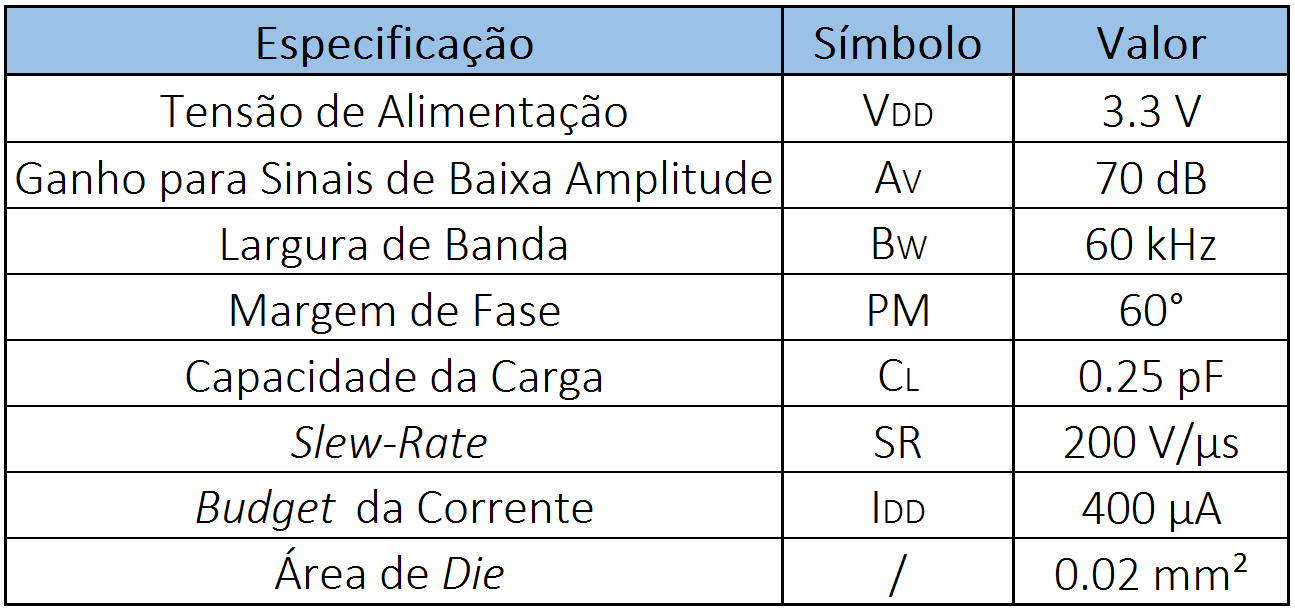
\includegraphics[keepaspectratio=true, scale=0.45]{teoricas/tabela1}
\end{table}

O circuito de ponto de partida para a realização do projecto é apresentado de seguida.

\begin{figure}[H]
	\centering
	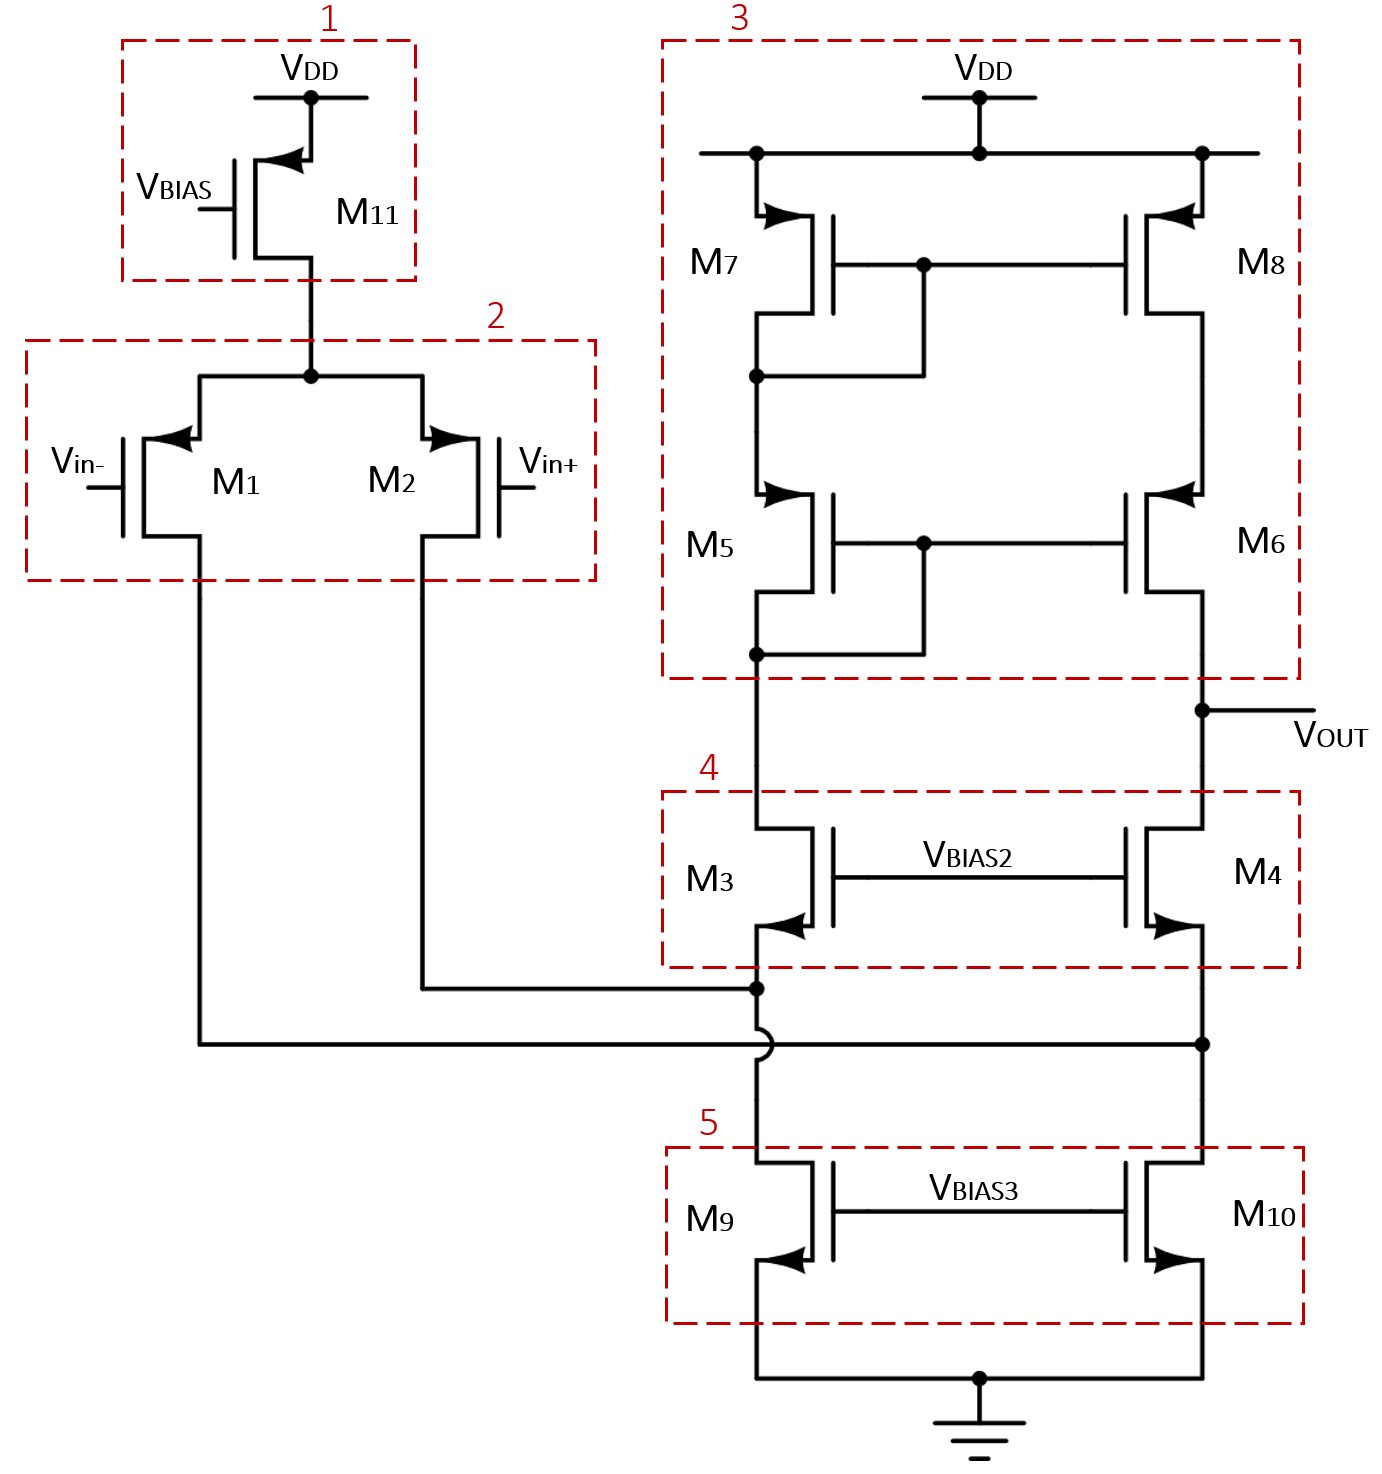
\includegraphics[keepaspectratio=true, scale=0.50]{teoricas/circuito1}
	\vspace{-0.5em}
	\caption{Circuito do amplificador a projectar.}
	\vspace{-0.8em}
\end{figure} 

\pagebreak

\section{Funcionamento Teórico do Circuito}

O circuito a desenvolver é do tipo \textit{folded cascode} CMOS OTA (\textit{Operational Transconductance Amplifier}). Os amplificadores OTA são caracterizados por apresentar ganhos e valores de impedância de saída elevados. O valor elevado da impedância de saída  faz com que sejam especialmente indicados para cargas capacitivas podendo, no entanto, servir para cargas resistivas pequenas através de \textit{feedback}.

Quando se compara o \textit{folded cascode} com o \textit{telescopic} observa-se que se tem o dobro da corrente e ganhos muito similares. No entanto, deve-se notar que se tem melhor largura de banda, \textit{slew-rate}, estabilidade e impedância de saída mais elevada. O compromisso por estas qualidades é uma velocidade de resposta inferior, assim como índices de ruido superiores e uma pior resposta na frequência.

Analisando o circuito da Figura 1 em pormenor identificam-se 5 blocos, sendo importante analisar a função de cada um, para que melhor se possa compreender o funcionamento e comportamento do circuito na sua totalidade. O Bloco 1 representa o transístor responsável pela polarização do circuito. O Bloco 2 representa um par diferencial PMOS. O Bloco 3 corresponde a um espelho de corrente \textit{cascode} básico do tipo PMOS. O Bloco 4 actua como isolamento. O Bloco 5 funciona como fonte de corrente que ``puxa'' sempre $I$ (corrente de M\textsubscript{11}) para o \textit{ground}.

Relativamente ao par diferencial, o circuito pode funcionar de acordo com três situações:

\begin{itemize}
	\vspace{-3mm}
	\item $v_{in-} = v_{in+} \rightarrow$ situação 1
	\vspace{-1.5mm}
	\item $v_{in-} > v_{in+} \rightarrow$ situação 2
	\vspace{-1.5mm}
	\item $v_{in-} < v_{in+} \rightarrow$ situação 3
\end{itemize}

Na situação 1, cada transístor do par diferencial, M\textsubscript{1} e M\textsubscript{2}, tem metade da corrente que passa em M\textsubscript{11} e o circuito apresenta o seguinte comportamento.

\begin{figure}[H]
	\centering
	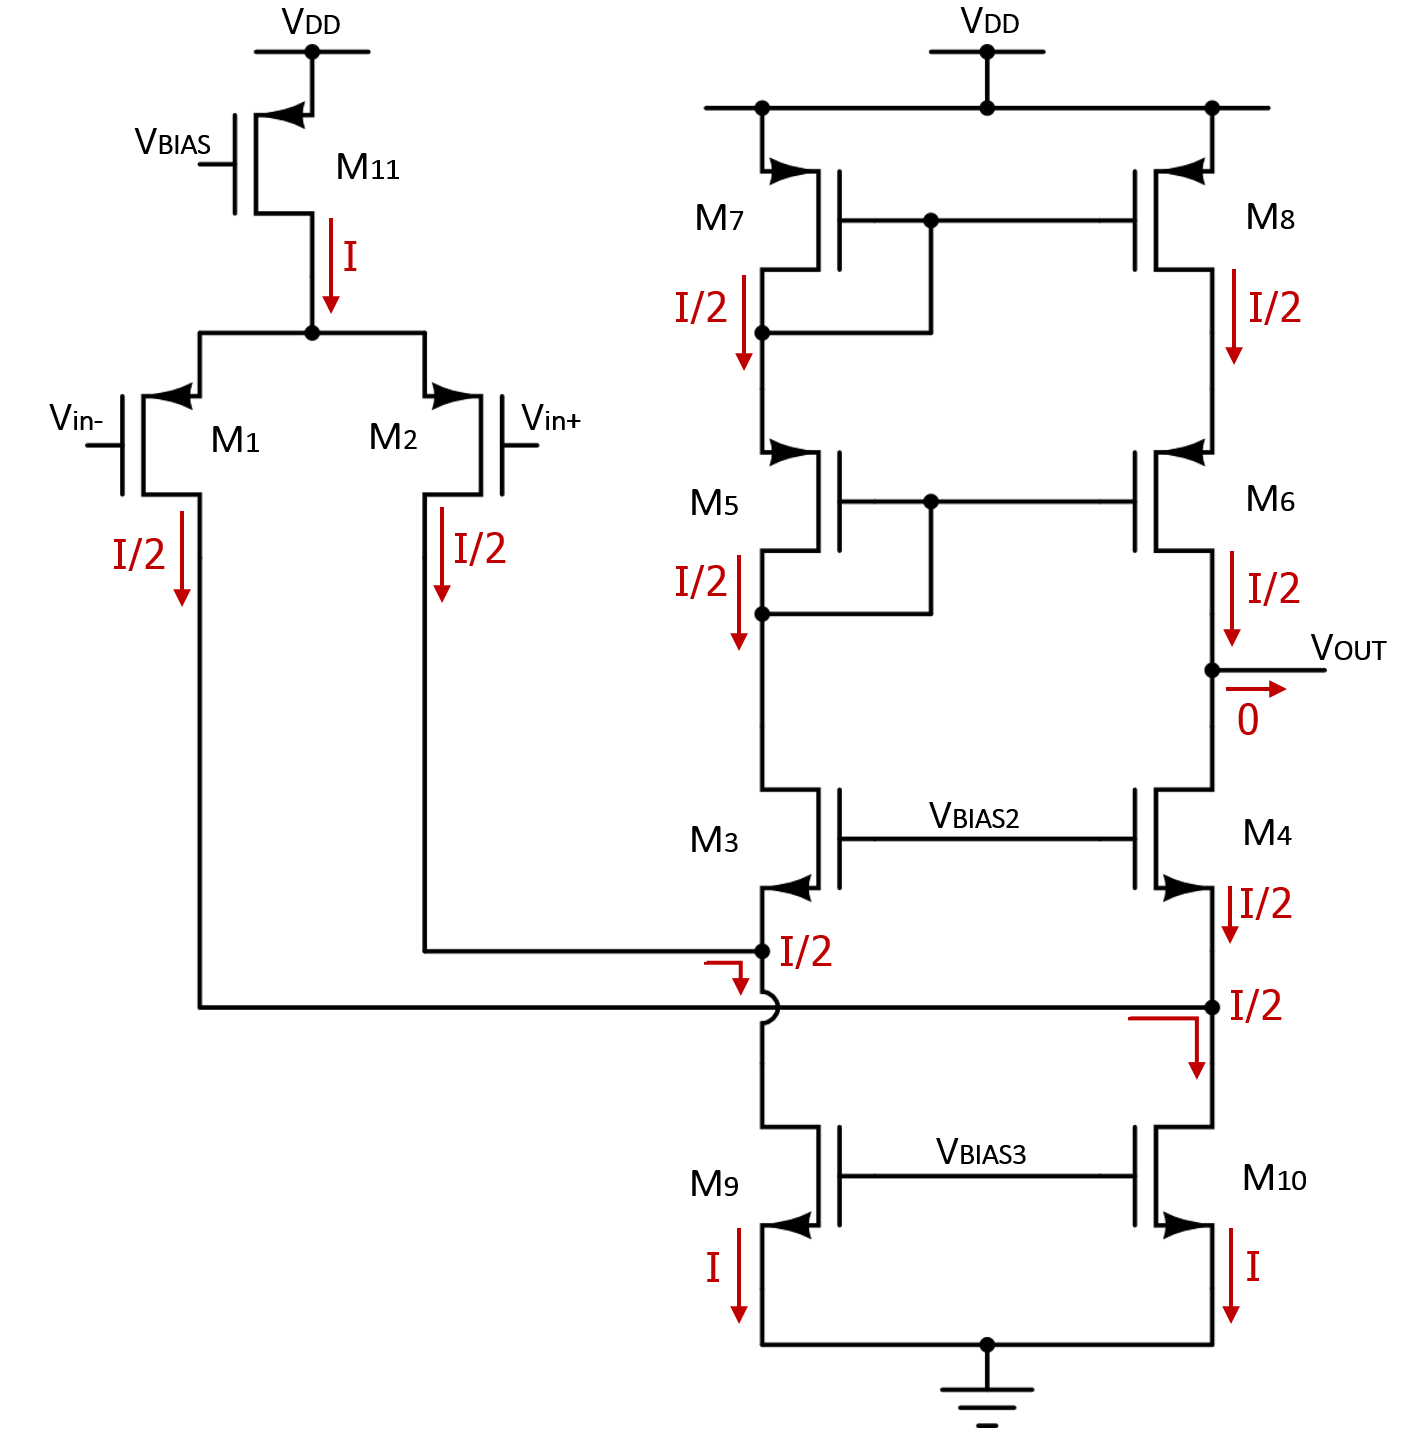
\includegraphics[keepaspectratio=true, scale=0.47]{teoricas/situacao1}
	\vspace{-0.5em}
	\caption{Funcionamento do circuito na situação 1.}
	\vspace{-0.8em}
\end{figure} 

Considerando agora o extremo da situação 2, a tensão na \textit{gate} de M\textsubscript{1} toma o valor máximo da fonte de tensão que polariza esse transístor e a tensão na \textit{gate} de M\textsubscript{2} é nula. Assim, o circuito apresenta o seguinte comportamento.

\begin{figure}[H]
	\centering
	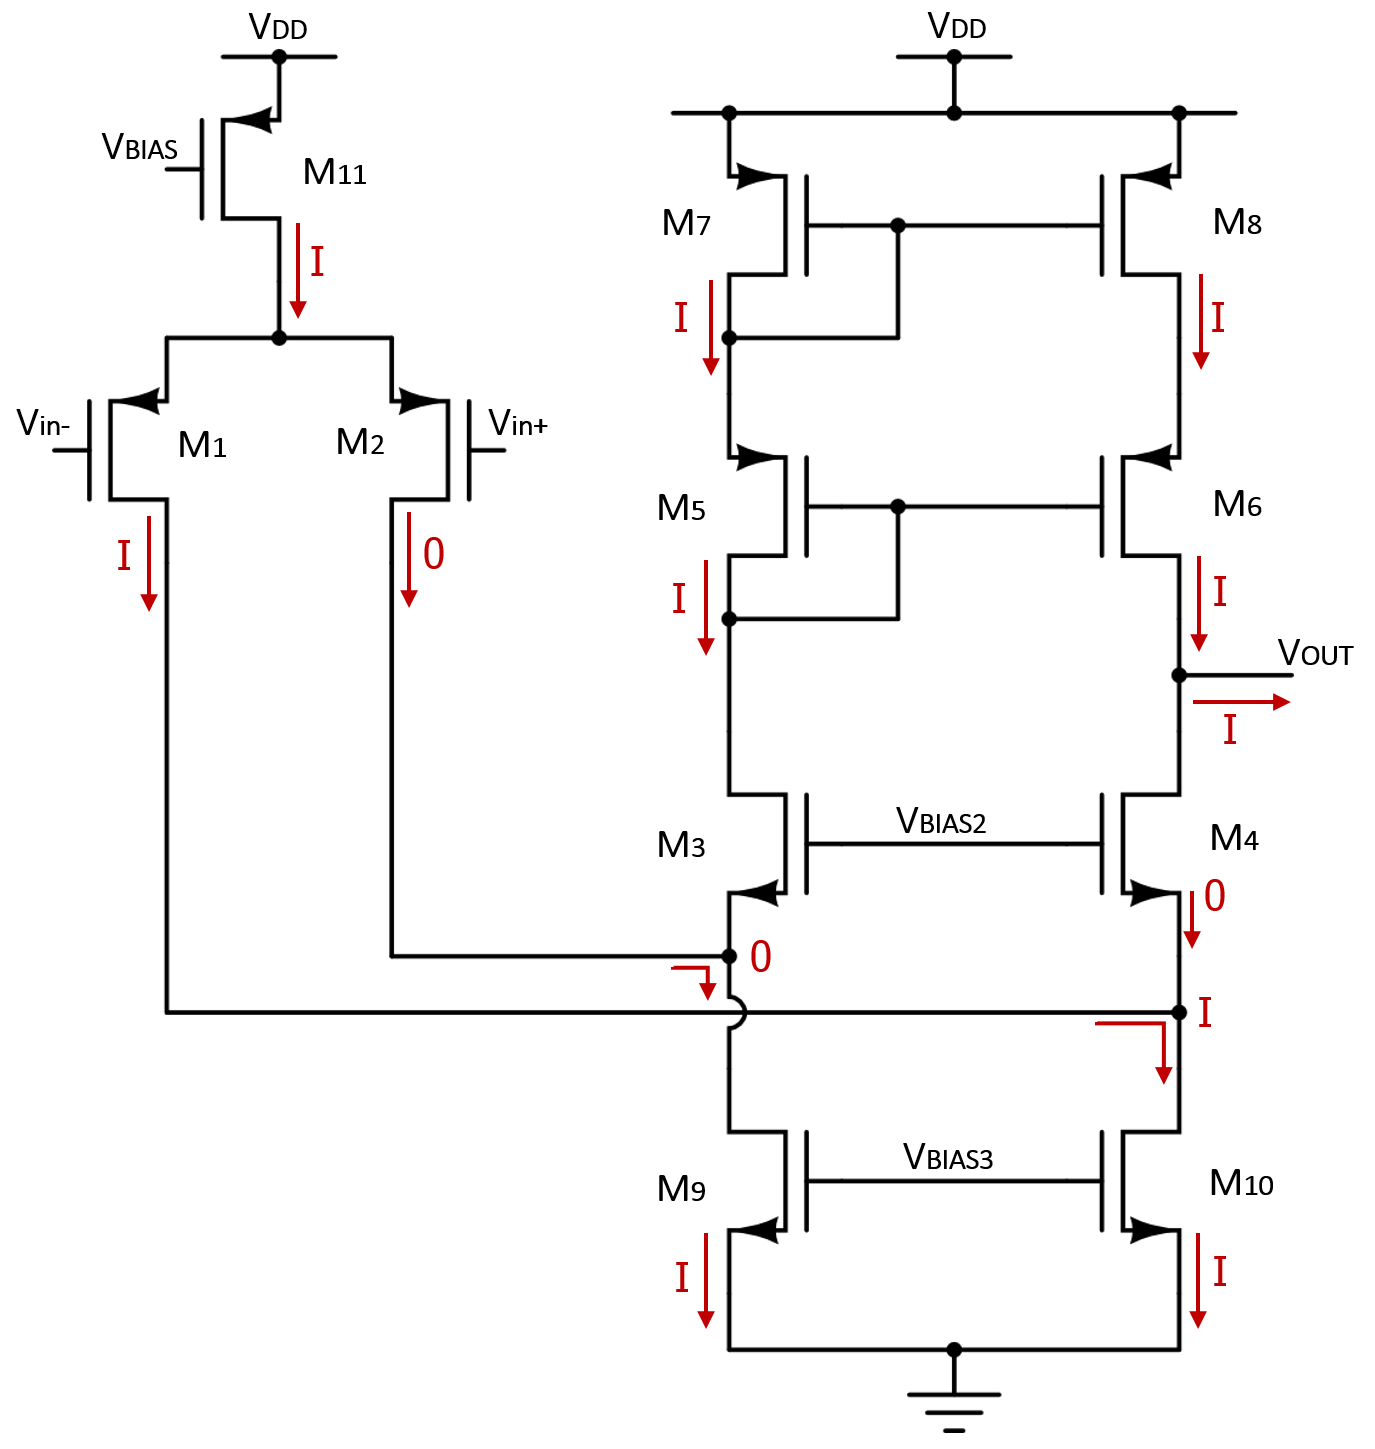
\includegraphics[keepaspectratio=true, scale=0.47]{teoricas/situacao2}
	\vspace{-0.5em}
	\caption{Funcionamento do circuito no extremo da situação 2.}
	\vspace{-0.8em}
\end{figure} 

Considerando agora o extremo da situação 3, a tensão na \textit{gate} de M\textsubscript{2} toma o valor máximo da fonte de tensão que polariza esse transístor e a tensão na \textit{gate} de M\textsubscript{1} é nula. Assim, o circuito apresenta o seguinte comportamento.

\begin{figure}[H]
	\centering
	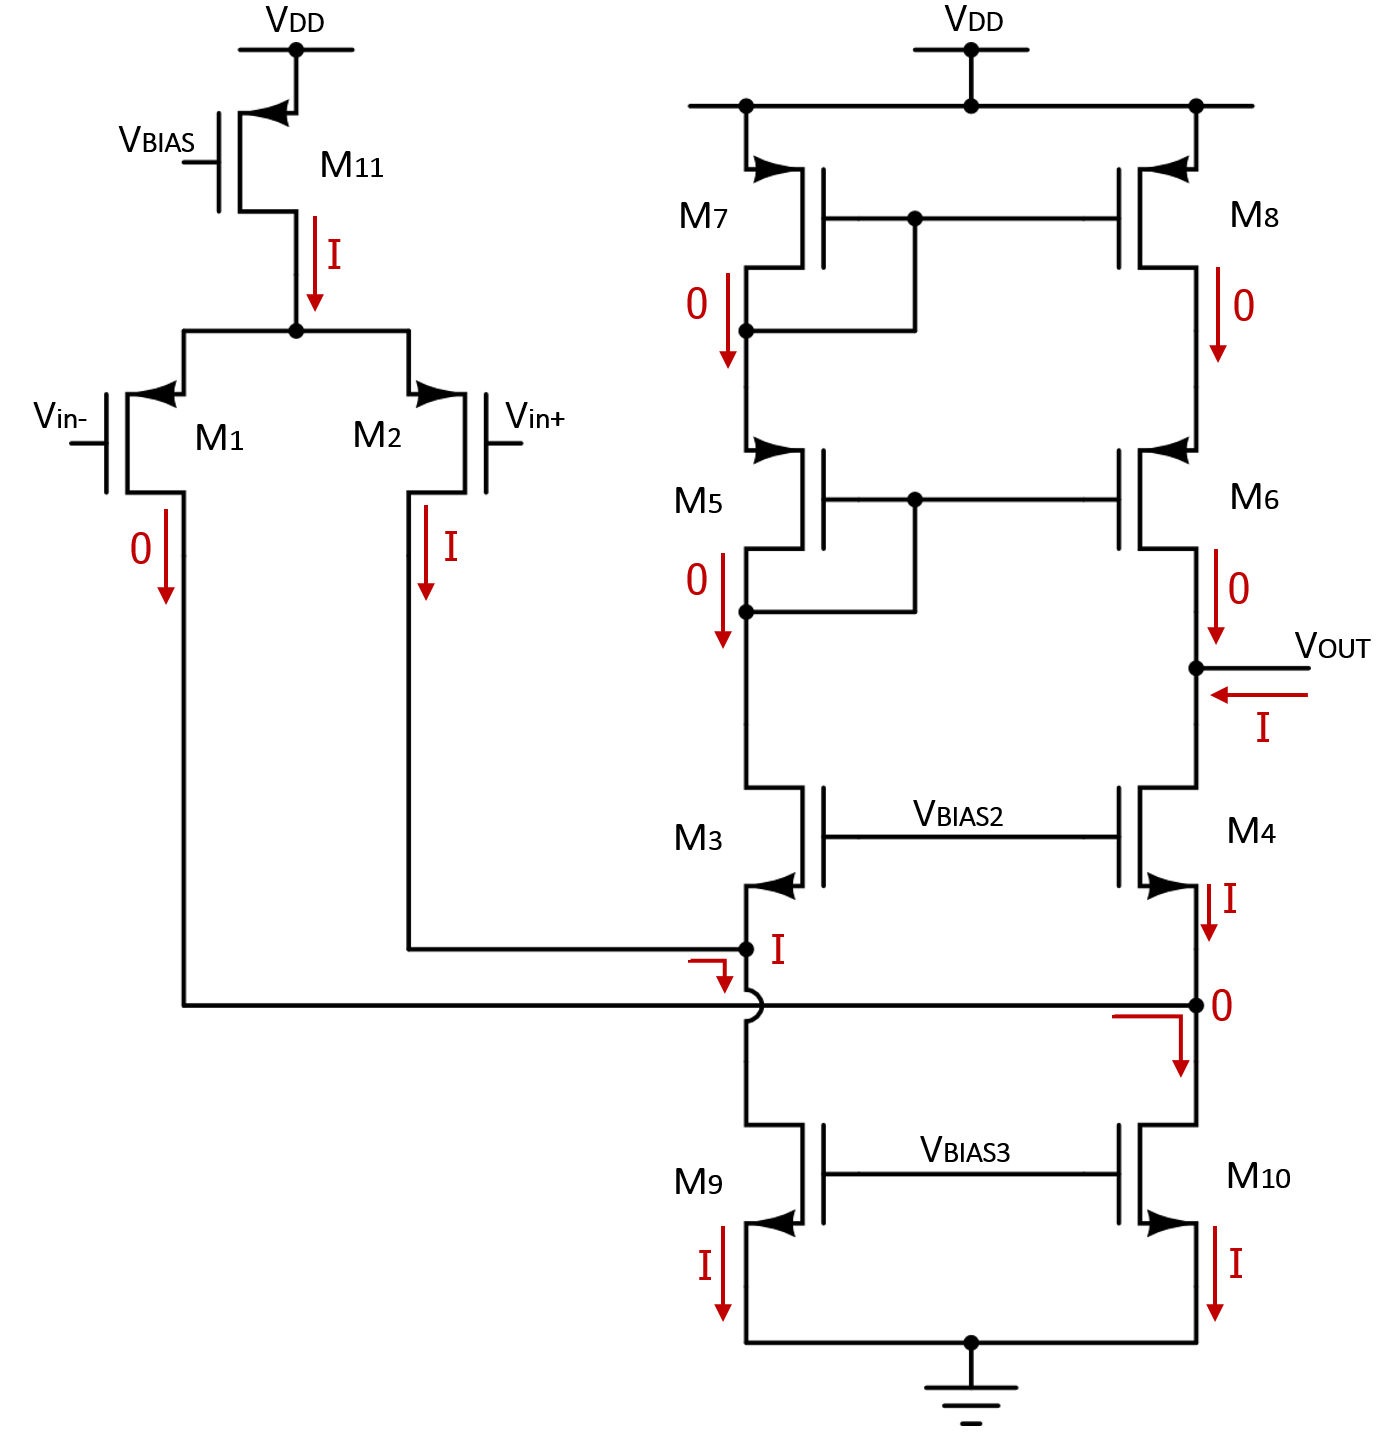
\includegraphics[keepaspectratio=true, scale=0.47]{teoricas/situacao3}
	\vspace{-0.5em}
	\caption{Funcionamento do circuito no extremo da situação 3.}
	\vspace{-0.8em}
\end{figure} 

\section{Dimensionamento dos Transístores}

A primeira fase no projecto do amplificador passou por decidir as dimensões dos vários transístores. Sabe-se que a dimensão de um transístor é dada pelos parâmetros $W$ (\textit{width} - largura) e $L$ (\textit{lenght} - comprimento). 

\subsection{\textit{Slew-Rate}}

Para efectuar o primeiro dimensionamento dos transístores teve-se em consideração o critério da \textit{slew-rate}, onde se pretende atingir um valor de 200 V/$\mu$s.

O valor de $L$ ficou decidido à partida como sendo 1 $\mu$m para todos os transístores do circuito, isto porque se tem como \textit{rule of thumb} que, para se evitar o efeito de modulação do comprimento do canal, o valor de $L$ deve ser maior ou igual a 1 $\mu$m. O valor de $W$ pode ser calculado recorrendo à equação que determina a corrente num transístor. Para um transístor do tipo P a corrente é dada por

\vspace{-3mm}
\begin{equation}
I_{D} = \frac{1}{2}\mu_{n}C_{ox}\times \left(\frac{W}{L}\right) \times \left(V_{GS}-V_{TH}\right)^2 = k_P \times \left(\frac{W}{L}\right) \times V_{OD}^2,
\label{eq:corrente}
\end{equation}

\vspace{1mm}
sendo que para um transístor do tipo N troca o valor do factor de ganho, em vez de $k_P$ tem-se $k_N$.

Da equação anterior pretende-se determinar o valor de $W$ dos vários transístores, sendo então necessário saber o valor de $L$ (já determinado anteriormente), o valor da corrente que passa nos transístores, $I_{D}$, o valor de $k$ e o valor da tensão de \textit{overdrive}, $V_{OD}$.

O valor da tensão de \textit{overdrive} definiu-se como sendo de 0.2 V para todos os transístores. Este valor deriva de outra \textit{rule of thumb} que indica que se deve escolher para $V_{OD}$ um valor de 0.2V - menos do que isso e fica-se demasiado sensível a $V_{TH}$ e mais do que isso e fica-se com pouca margem de saturação, que é uma medida do quão dentro da saturação se está, sendo calculada por $V_{DS} - V_{OD}$.

O valor de $k$ pode ser obtido com recurso aos \textit{process parameters}, sendo de referir que o valores que se retiram das \textit{datasheets} representam apenas $\mu_{n}C_{ox}$, pelo que têm de ser multiplicados por $1/2$ para que se obtenha o factor de ganho final, como se pode ver na próxima equação, para o caso de um transístor do tipo P:

\vspace{-3mm}
\begin{equation}
k_P = \frac{1}{2}\mu_{n}C_{ox} = \frac{1}{2} \times KP_P.
\end{equation}

\vspace{1mm}
Os valores já conhecidos que ajudam a obter o valor de $W$ através da equação (2.1) encontram-se esquematizados na seguinte tabela.

\begin{table}[H]
	\centering
	\caption{Valores especificados para algumas das características que definem os transístores.}
	\vspace{-1.5mm}
	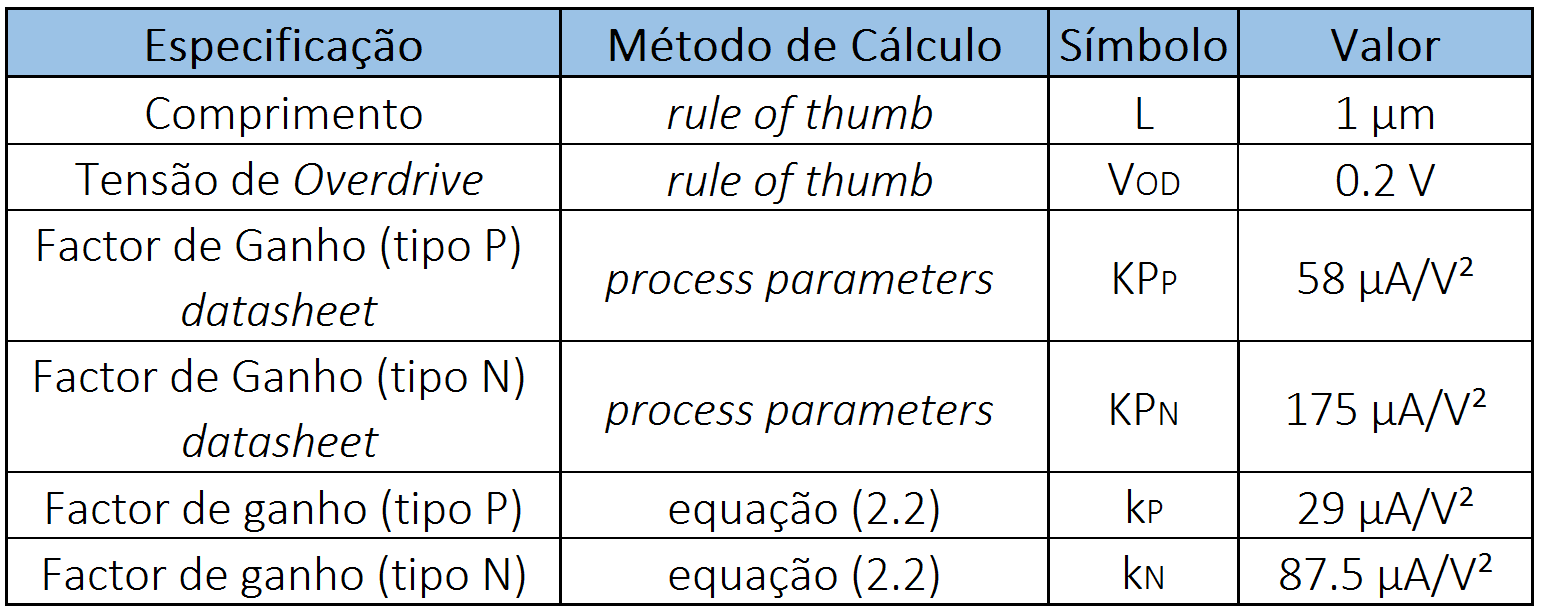
\includegraphics[keepaspectratio=true, scale=0.45]{teoricas/tabela2}
\end{table}

Para determinar os valores das correntes que passam nos vários transístores começou-se por determinar a corrente máxima à saída do circuito. Existe uma relação entre a \textit{slew-rate}, SR, e a corrente de saída máxima, $I_{out_{max}}$ expressa por

\vspace{-3mm}
\begin{equation}
\text{SR} = \frac{I_{out_{max}}}{C_L},
\end{equation}

\vspace{1mm}
que nos permite concluir que quanto maior for a corrente de saída, mais depressa é carregado o condensador que constitui a carga.

Com os valores da Tabela 1 obtém-se:

\vspace{-3mm}
\begin{equation}
\text{SR} = \frac{I_{out_{max}}}{C_L} \leftrightarrow I_{out_{max}} = 200 \times 0.25 \times 10^{-6}~\text{A} = 50~\mu \text{A}.
\end{equation}

\vspace{1mm}
Analisando as Figuras 3 a 4 percebe-se que a corrente $I_{out_{max}}$ corresponde a $I/2$, pelo que o valor máximo de $I$ corresponde a 100 $\mu$A. O dimensionamento dos transístores foi feito tendo em conta o ponto de funcionamento em repouso (PFR), situação 1, de acordo com

\vspace{-3mm}
\begin{equation}
W_P  = \frac{I_{D} \times L}{k_P \times V_{OD}^2} \rightarrow \text{transístor tipo PMOS};
\end{equation}
\vspace{1mm}
\begin{equation}
W_N  = \frac{I_{D} \times L}{k_N \times V_{OD}^2} \rightarrow \text{transístor tipo NMOS}.
\end{equation}

\vspace{1mm}
Os valores obtidos para a \textit{width} dos vários transístores apresenta-se na tabela seguinte. De notar que os valores foram arredondados ao inteiro mais próximo.

\begin{table}[H]
	\centering
	\caption{Valores de $W$ dos transístores que constituem o circuito, calculados em função do PFR.}
	\vspace{-1.5mm}
	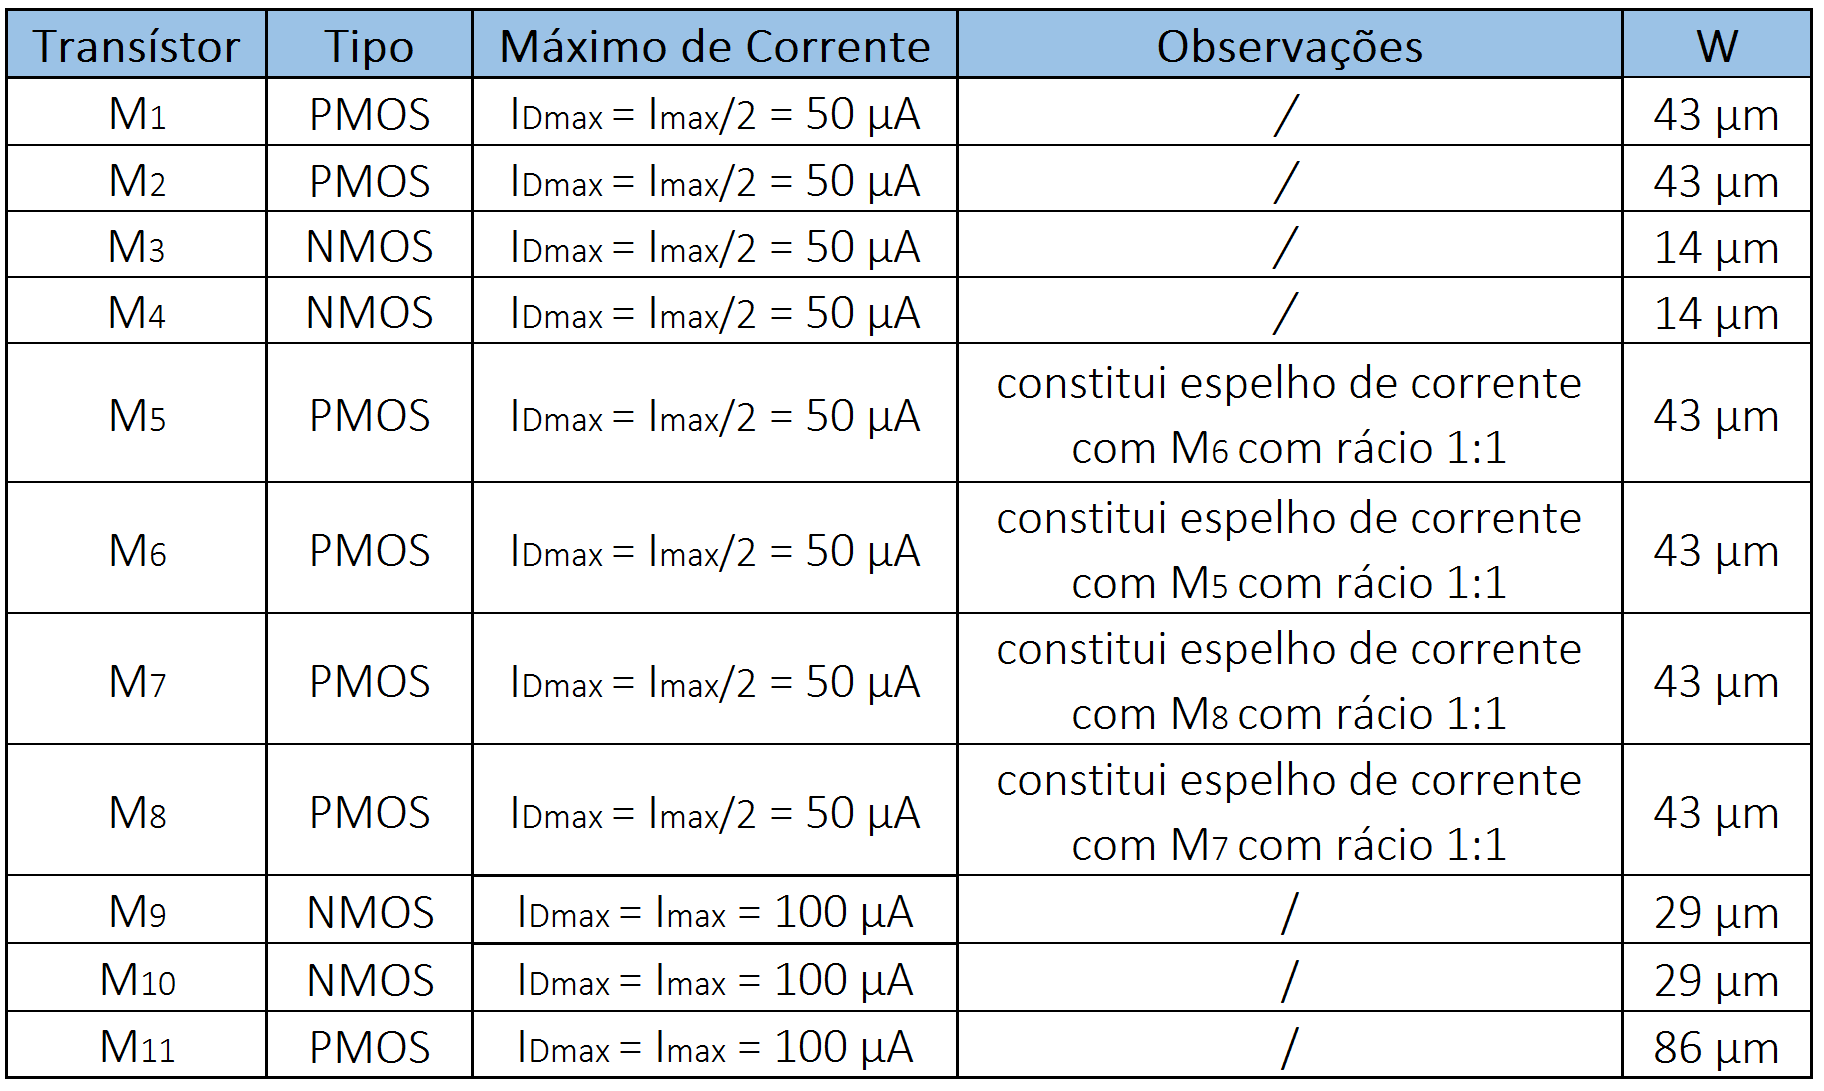
\includegraphics[keepaspectratio=true, scale=0.45]{teoricas/valoresW2}
\end{table}

De referir que os transístores M\textsubscript{5} e M\textsubscript{6} têm as mesmas dimensões, tal como pretendido, pois formam um espelho de corrente que tem como rácio 1:1. O mesmo se aplica aos transístores M\textsubscript{7} e M\textsubscript{8}.

Com o dimensionamento dos transístores feito procede-se a uma primeira simulação do circuito, com o intuito de verificar o seu funcionamento. Porém, antes de simular o circuito alterou-se a sua polarização, para que em vez de ser feita em tensão seja feita em corrente. Isto é feito porque uma polarização em corrente permite ter mais controlo, sendo que quando é feita em tensão não se tem garantias dos valores pretendidos.  

Assim, o circuito da Figura 1 foi alterado para o apresentado de seguida.

\begin{figure}[H]
	\centering
	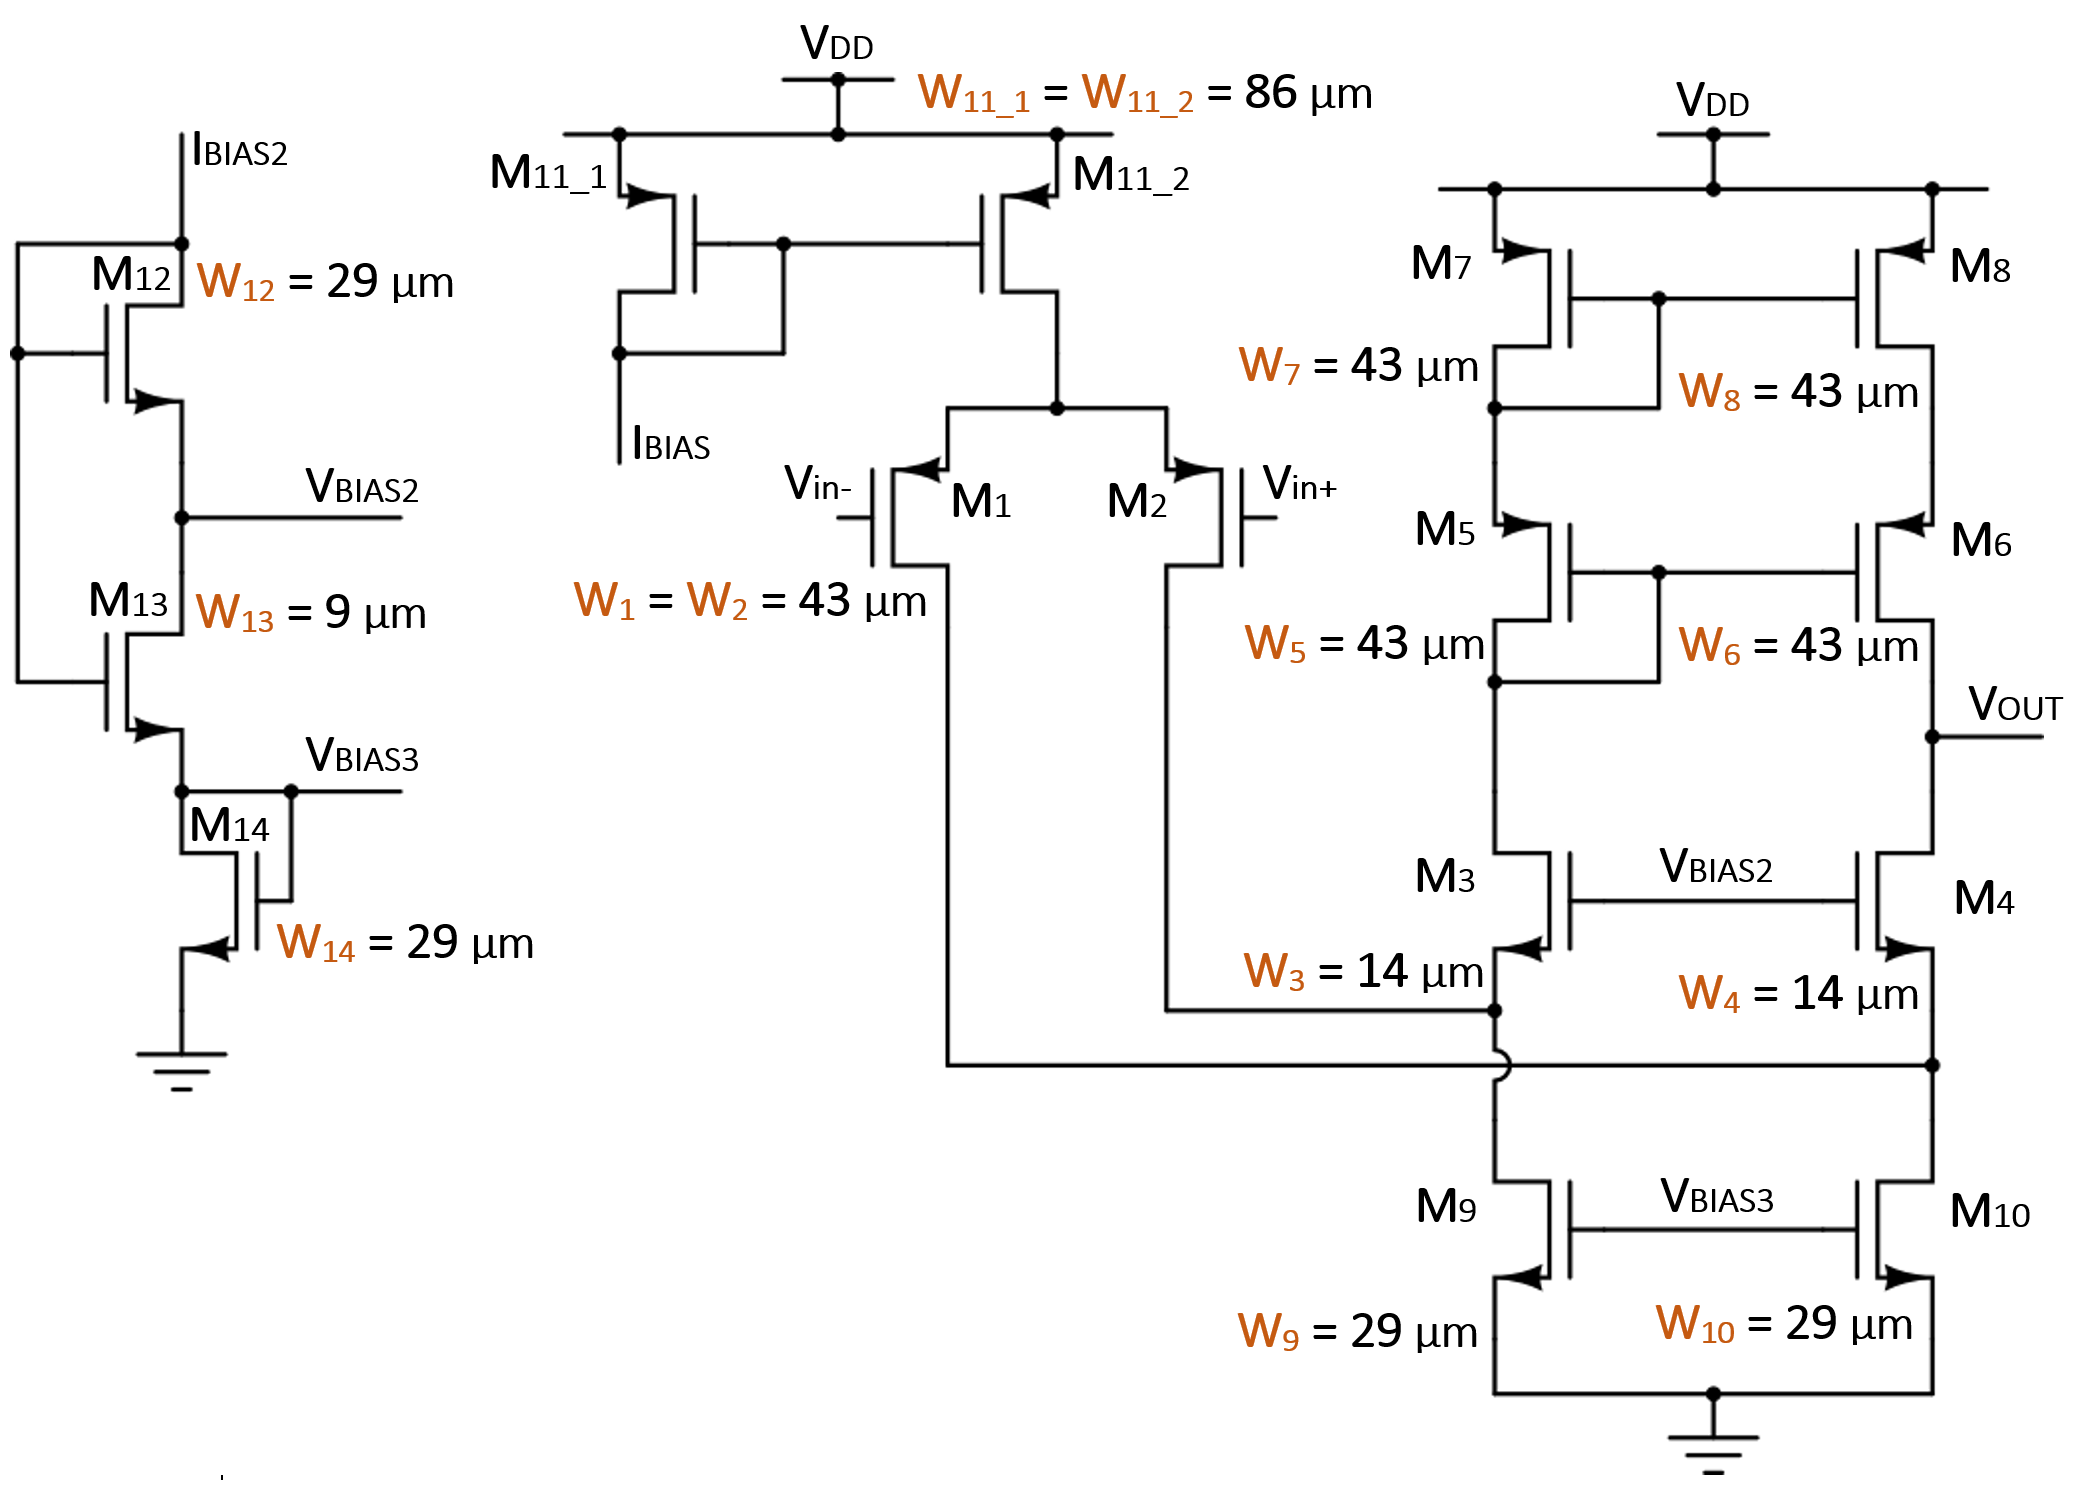
\includegraphics[keepaspectratio=true, scale=0.55]{teoricas/primeirasimul}
	\vspace{-0.5em}
	\caption{Primeiro circuito de simulação do amplificador.}
	\vspace{-0.8em}
\end{figure} 

Na figura anterior pode-se ver o valor de $W$ utilizado nos vários transístores, sendo que para todos o valor de $L$ é de 1 $\mu$m.

Como se pode ver, o transístor M\textsubscript{11} que é originalmente polarizado em tensão com $V_{BIAS}$, Bloco 1, foi substituído por um espelho de corrente básico que é polarizado em corrente com $I_{BIAS}$. A polarização feita com recurso a $V_{BIAS_{2}}$ e $V_{BIAS_{3}}$ foi tanbém alterada para passar a ser feita em corrente com $I_{BIAS_{2}}$, através de um espelho de corrente \textit{cascode} \textit{low-voltage}. O valor de $I_{BIAS}$ e de $I_{BIAS_{2}}$ é de 100 $\mu$A.

De notar que os transístores M\textsubscript{11\textsubscript{1}} e M\textsubscript{11\textsubscript{2}} têm a mesma dimensão que aquela que foi determinada para M\textsubscript{11}, uma vez que a corrente que os atravessa é também 100 $\mu$A e são do tipo PMOS. Já os transístores M\textsubscript{12} e M\textsubscript{14} têm a mesma dimensão que M\textsubscript{9} e M\textsubscript{10}, uma vez que a corrente que os atravessa é também 100 $\mu$A e são do tipo NMOS. O transístor M\textsubscript{13}, de acordo com o funcionamento teórico de um espelho de corrente \textit{cascode} \textit{low-voltage}, deve ter um $W$ 3 vezes inferior ao de M\textsubscript{12}, assim como deve funcionar sempre no tríodo, o que implica uma \textit{width} de 9 $\mu$m.

Na Figura 6 encontra-se o \textit{schematic} criado no Cadence correspondente ao da Figura 5.

\begin{figure}[H]
	\centering
	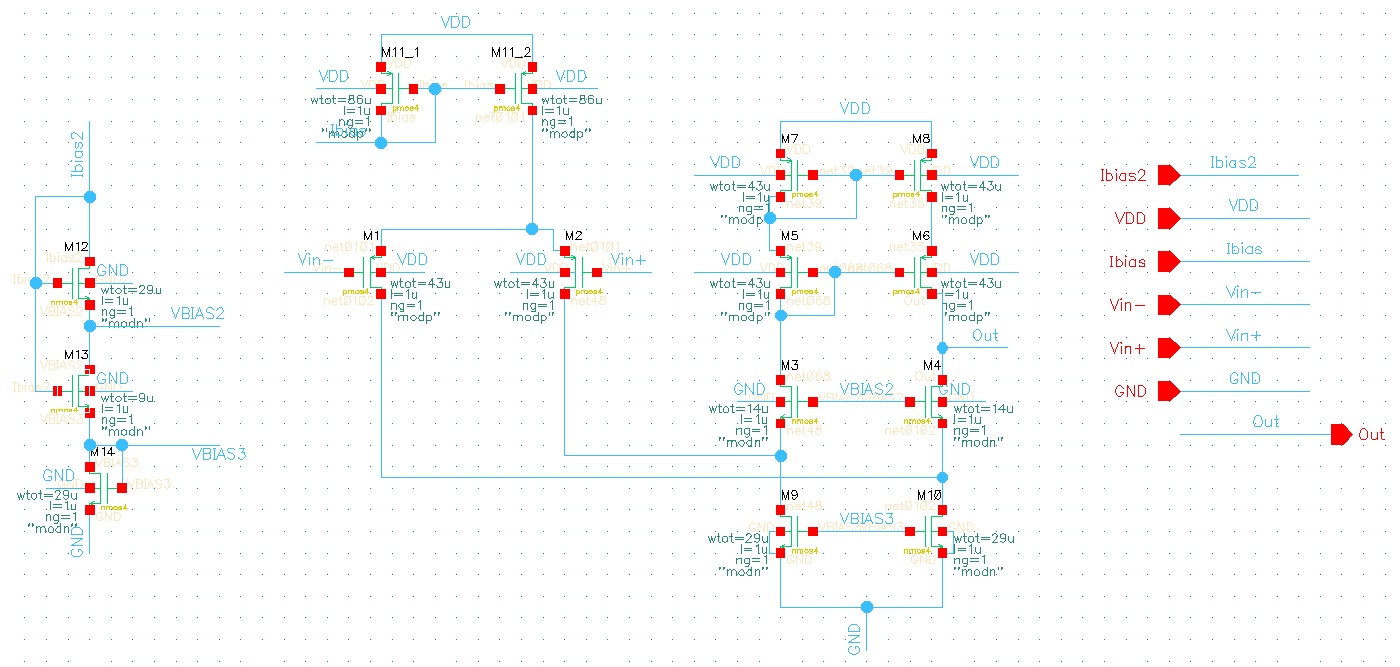
\includegraphics[keepaspectratio=true, scale=0.80]{exps/Woriginais}
	\vspace{-0.5em}
	\caption{\textit{Schematic} do circuito criado para a primeira simulação.}
	\label{fig:schematic1}
	\vspace{-0.8em}
\end{figure} 

Com o \textit{schematic} anterior projectou-se um símbolo e criaram-se novos \textit{schematics} de \textit{testbench}, como se pode ver nas Figura 7, 8 e 9.

\vspace{3mm}

\begin{figure}[H]
	\centering
	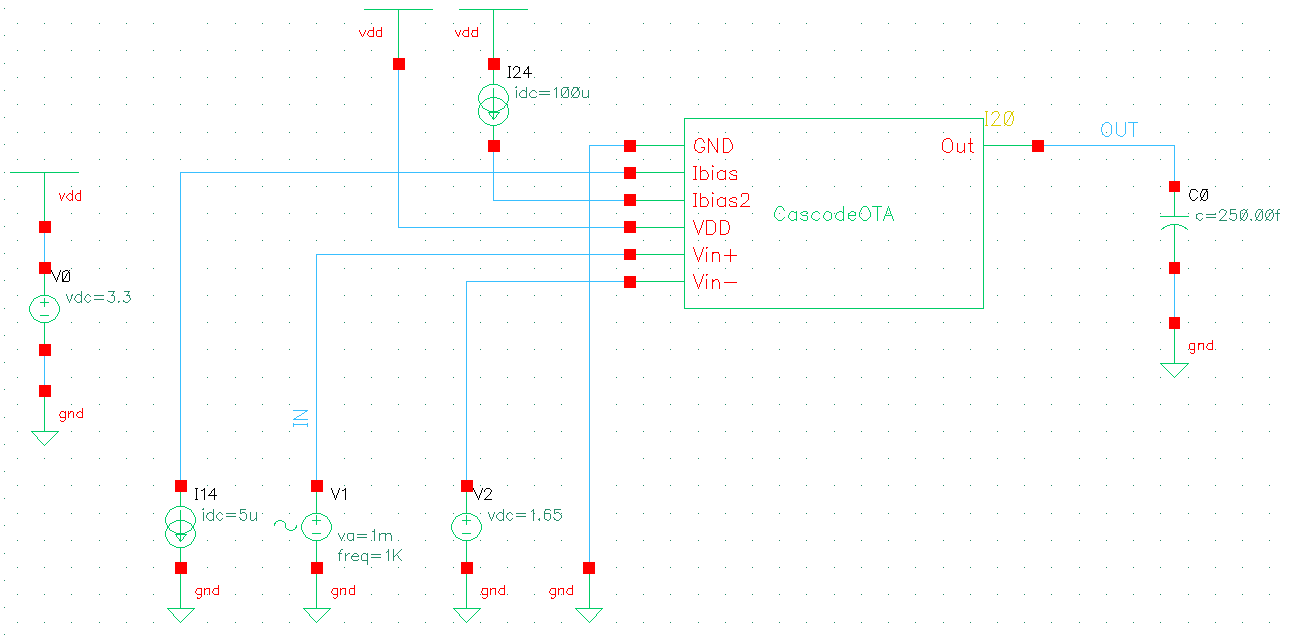
\includegraphics[keepaspectratio=true, scale=0.60]{exps/TBdctrans}
	\vspace{-0.5em}
	\caption{\textit{Schematic} do \textit{testbench} que permite simular o circuito em testes transiente e de resposta DC.}
	\vspace{-0.8em}
\end{figure} 

\vspace{4mm}

\begin{figure}[H]
	\centering
	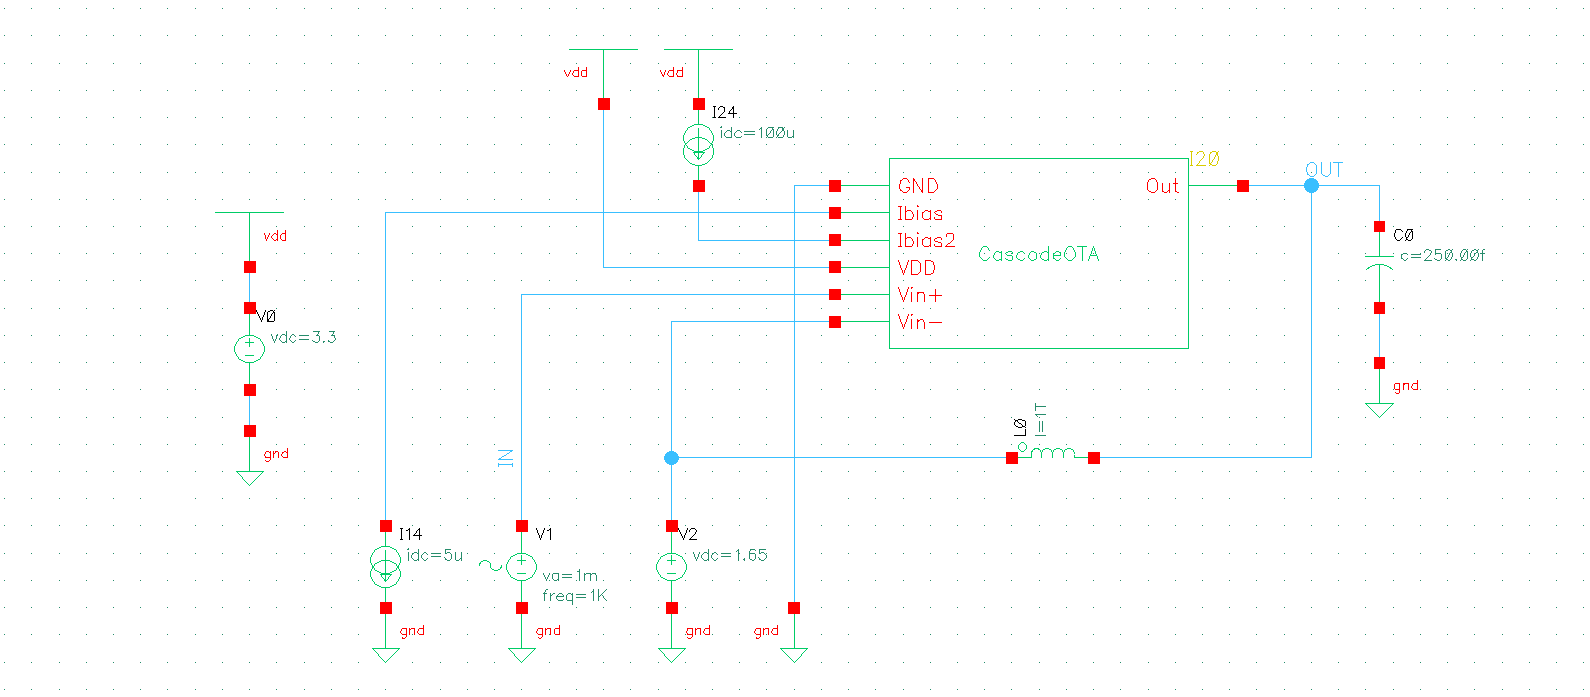
\includegraphics[keepaspectratio=true, scale=0.60]{exps/TBac}
	\vspace{-0.5em}
	\caption{\textit{Schematic} do \textit{testbench} que permite simular o circuito em testes de resposta AC.}
	\vspace{-0.8em}
\end{figure} 

\begin{figure}[H]
	\centering
	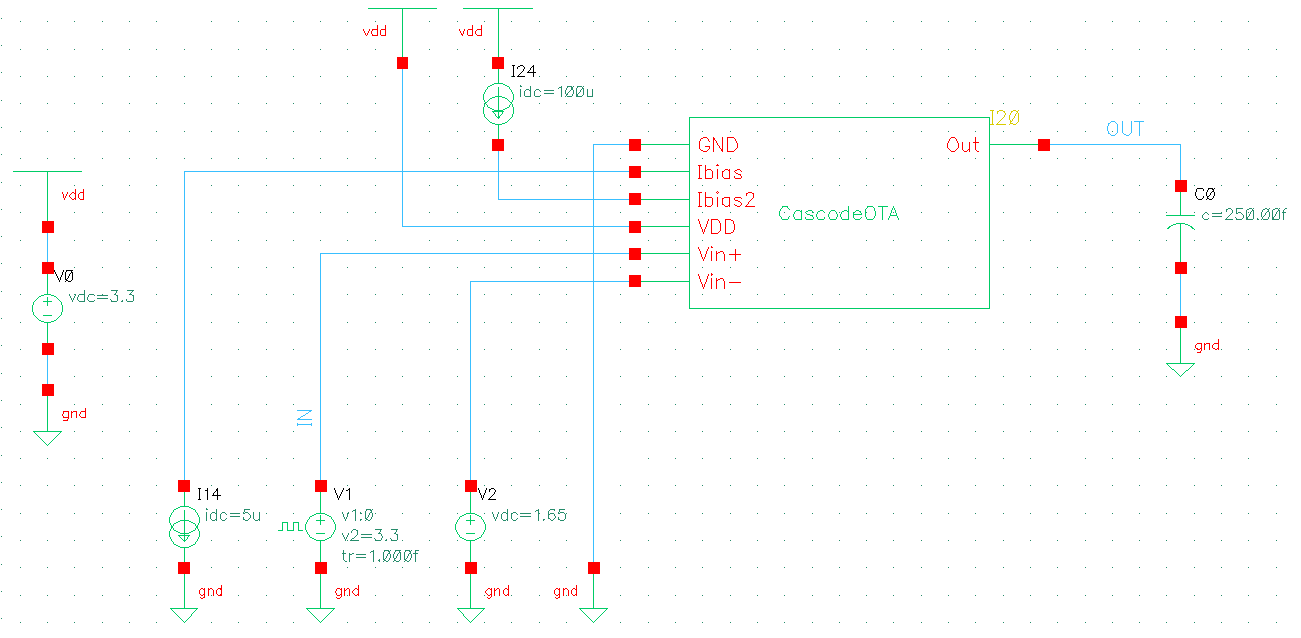
\includegraphics[keepaspectratio=true, scale=0.60]{exps/TBslewrate}
	\vspace{-0.5em}
	\caption{\textit{Schematic} do \textit{testbench} que permite simular o circuito em testes da \textit{slew-rate}.}
	\vspace{-0.8em}
\end{figure} 

Recorrendo ao circuito da Figura 7 efectuou-se uma análise transiente durante 2 ms. Para verificar se o circuito funciona como pretendido otpou-se por verificar se todos os transístores do amplificador tem a corrente $I_D$ pretendida, ou seja, de acordo com a Figura 1, e se estão na região de saturação.

\begin{figure}[H]
	\centering
	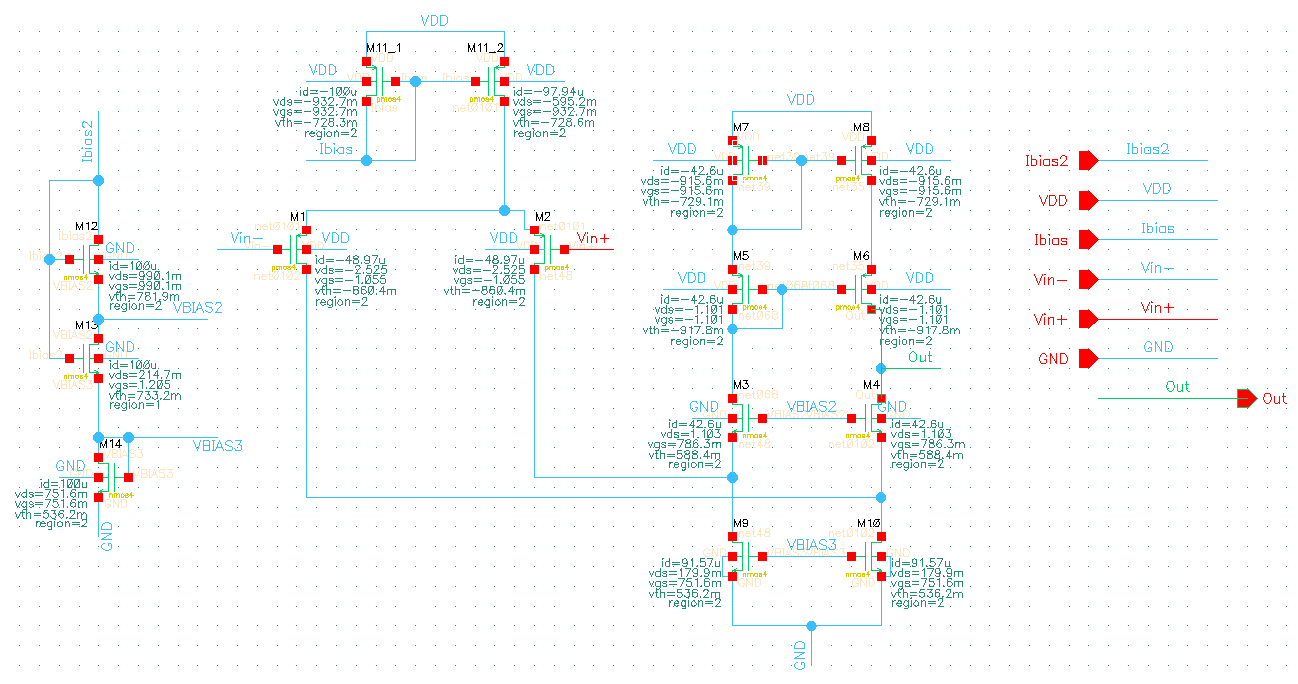
\includegraphics[keepaspectratio=true, scale=0.85]{exps/PFRoriginaisVTH}
	\vspace{-0.5em}
	\caption{Valores do PFR do \textit{schematic} da Figura \ref{fig:schematic1}.}
	\label{fig:PFR1}
	\vspace{-0.8em}
\end{figure} 

A região de funcionamento dos transístores pode ser vista na secção \textit{region}: 0 implica que o transístor está ao corte, 1 que está no tríodo, 2 que está na zona de saturação e 3 na região de \textit{subthreshold}.

Como se pode ver, todos os transístores do amplificador estão na região 2, tal como pretendido, assim como os que polarizam através de $I_{BIAS}$. Os transístores M\textsubscript{12} e M\textsubscript{14} do espelho de corrente \textit{cascode} \textit{low-voltage} estão também saturados e o transístor M\textsubscript{13} está no tríodo, tal como se queria.

Porém, apesar de os transístores estarem a funcionar na zona correcta, o valor das suas correntes está ligeiramente afastado do pretendio. Os transístores M\textsubscript{3}, M\textsubscript{4}, M\textsubscript{5}, M\textsubscript{6}, M\textsubscript{7} e M\textsubscript{8} deveriam ter um valor de $I_D$ de 50 $\mu$A, sendo, no entanto, o valor registado pela simulação de 42.6 $\mu$A. Para os transístores M\textsubscript{9} e M\textsubscript{10} esperava-se um valor de $I_D$ de 100 $\mu$A, sendo, no entanto, o valor registado pela simulação de 91.57 $\mu$A. As correntes do espelho de corrente básico estão de acordo com o esperado, sendo que os transístores M\textsubscript{1} e M\textsubscript{2} têm um valor de corrente de 48.97 $\mu$A, um valor próximo do esperado de 50 $\mu$A.

Até agora, para efectuar o dimensionamento dos transístores o critério que se teve em consideração foi a \textit{slew-rate}. Assim, com recurso à calculadora do Cadence calculou-se o seu valor, sendo este de $170.7\times10^6$ V/segundo $\leftrightarrow 169.9$ V/$\mu$s. O valor pretendido é de 200 V/$\mu$s, verificando-se então alguma diferença entre os dois valores.

Relativamente aos valores de $V_{GS}$ para os vários transístores, os valores teóricos esperados foram calculados com base nos \textit{process parameters} da seguinte forma:

\vspace{-6mm}
\begin{equation}
V_{TH_{0_{P}}} \approx 0.6 V \rightarrow V_{GS} = V_{OD} + V_{TH_{N}} = 0.2 + 0.6 = 0.8 V \rightarrow \text{transístor tipo PMOS};
\end{equation}
\begin{equation}
V_{TH_{0_{N}}} \approx 0.5 V \rightarrow V_{GS} = V_{OD} + V_{TH_{N}} = 0.2 + 0.5 = 0.7 V \rightarrow \text{transístor tipo NMOS}.
\end{equation}

\vspace{1mm}
Na Figura \ref{fig:PFR1} pode-se verificar que certos transístores do amplificador sofrem de efeito de corpo, ou seja, não têm o \textit{bulk} à mesma tensão que a \textit{source}. Para transístores NMOS tal ocorre se a \textit{source} não estiver ligada a GND e, para transístores PMOS, se a \textit{source} não estiver ligada a VDD.

Quando um transístor sofre de efeito de corpo o seu valor de $V_{TH}$ desvia-se de $V_{TH_{0}}$ (tensão de limiar na ausência de efeito de corpo) e, como tal, a sua tensão $V_{GS}$ toma também valores diferentes. De facto, os transístores PMOS que sofrem de feito de corpo (M\textsubscript{1}, M\textsubscript{2}, M\textsubscript{5} e M\textsubscript{6}), quando comparados aos que não sofrem, apresentam uma tensão de limiar mais afastada do valor da equação (3.7).

Na tabela seguinte pode-se ver as especificações pretendidas e as que se verificam até ao momento, sendo que a verde se assinalam aquelas que se considera cumpridas e a vermelho aquelas que se pretende melhorar. É de referir que ainda não se tem em consideração o critério da área, pois essa é uma preocupação final.

\begin{table}[H]
	\centering
	\caption{Especificações actuais do circuito.}
	\vspace{-1.5mm}
	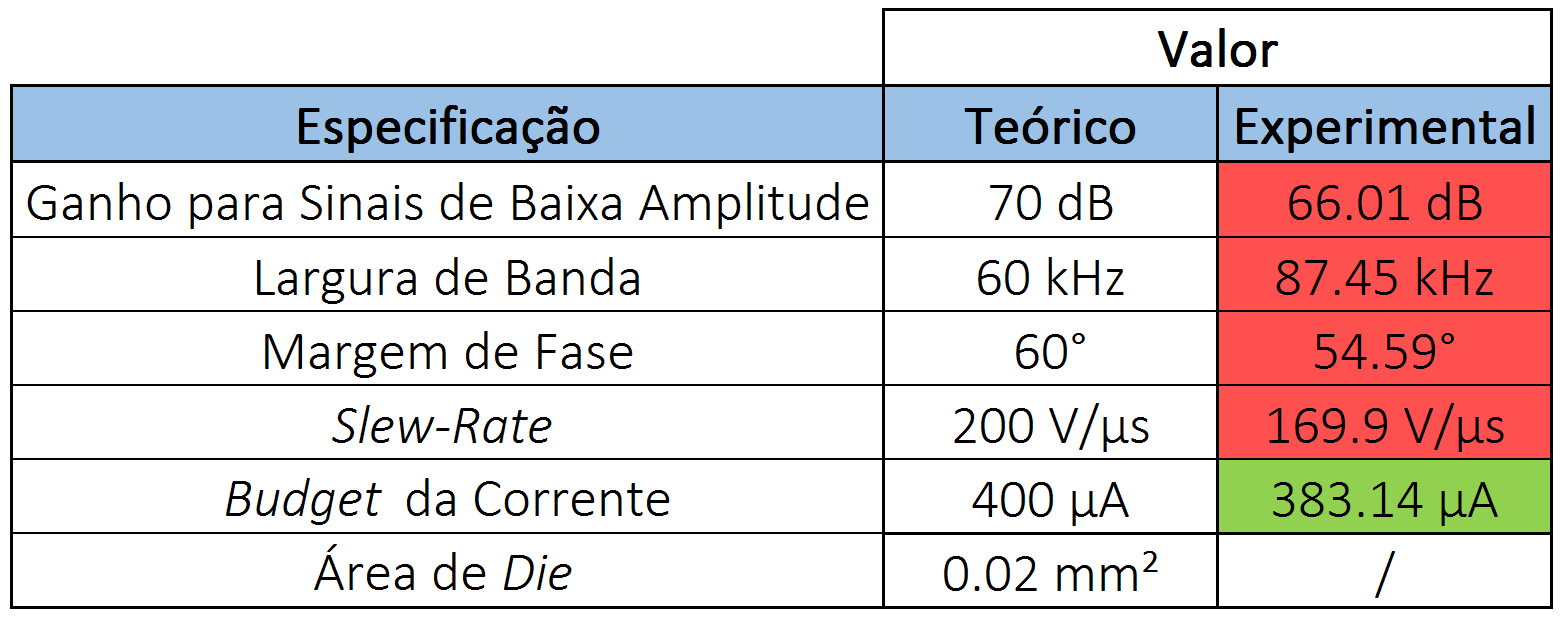
\includegraphics[keepaspectratio=true, scale=0.40]{teoricas/valoresoriginais}
\end{table}

Face à ligeira discrepância nos valores obtidos para a corrente nos vários transístores e para a \textit{slew-rate}, decidiu-se proceder a um ajuste nas dimensões dos transístores para se obter valores mais próximos dos esperados. Este ajuste foi feito ao nível dos transístores M\textsubscript{3} e M\textsubscript{4} pois, ao aumentar as suas dimensões faz-se variar as suas tensões $V_{GS}$, e como tal $V_{BIAS_{2}}$, o que resulta num aumento da tensão $V_{DS}$ de M\textsubscript{9}, que por sua vez faz aumentar a corrente daquele ramo.

O ajuste feito nesses dois transístores passou por aumentar o seu rácio $W/L$ para o dobro, ou seja, o valor de $W$ passou de 14 $\mu$m para 28 $\mu$m. À primeira vista não parecer ser um ajuste fino, no entanto, está associado à existência de um efeito de segunda-ordem.

De facto, quando se é mais criterioso, a corrente de um transístor não é calculada de acordo com a equação (2.1), mas sim de acordo com

\vspace{-3mm}
\begin{equation}
I_{D} = \frac{1}{2}\mu_{n}C_{ox}\times \left(\frac{W}{L}\right) \times \left(V_{GS}-V_{TH}\right)^2 \times \left(1+\lambda V_{DS}\right) = k_P \times \left(\frac{W}{L}\right) \times V_{OD}^2 \times \left(1+\lambda V_{DS}\right).
\end{equation}

\vspace{1mm}
Como se pode ver, sobre o valor da corrente existe um efeito de segunda-ordem com a introdução da parcela $\left(1+\lambda V_{DS}\right)$. Assim se explica que, quando o valor de $W$ de M\textsubscript{3} e M\textsubscript{4} passa para o dobro, a corrente nos transístores aumenta em aproximadamente 7$\mu$A, conseguindo-se obter o valor desejado de 50$\mu$A.

Fizeram-se mais ajustes finos nos transístores que polarizam o amplificador, sendo que o transístor M\textsubscript{12} passou para um $W$ de 28 $\mu$m e o transístor M\textsubscript{13} para um $W$ de 7 $\mu$m. Estes ajustes nos transístores foram feitos com o objectivo de melhorar a corrente dos respectivos ramos.

Na Figura \ref{fig:ajustefail} apresenta-se o circuito com o ajuste nas dimensões dos transístores.

\begin{figure}[H]
	\centering
	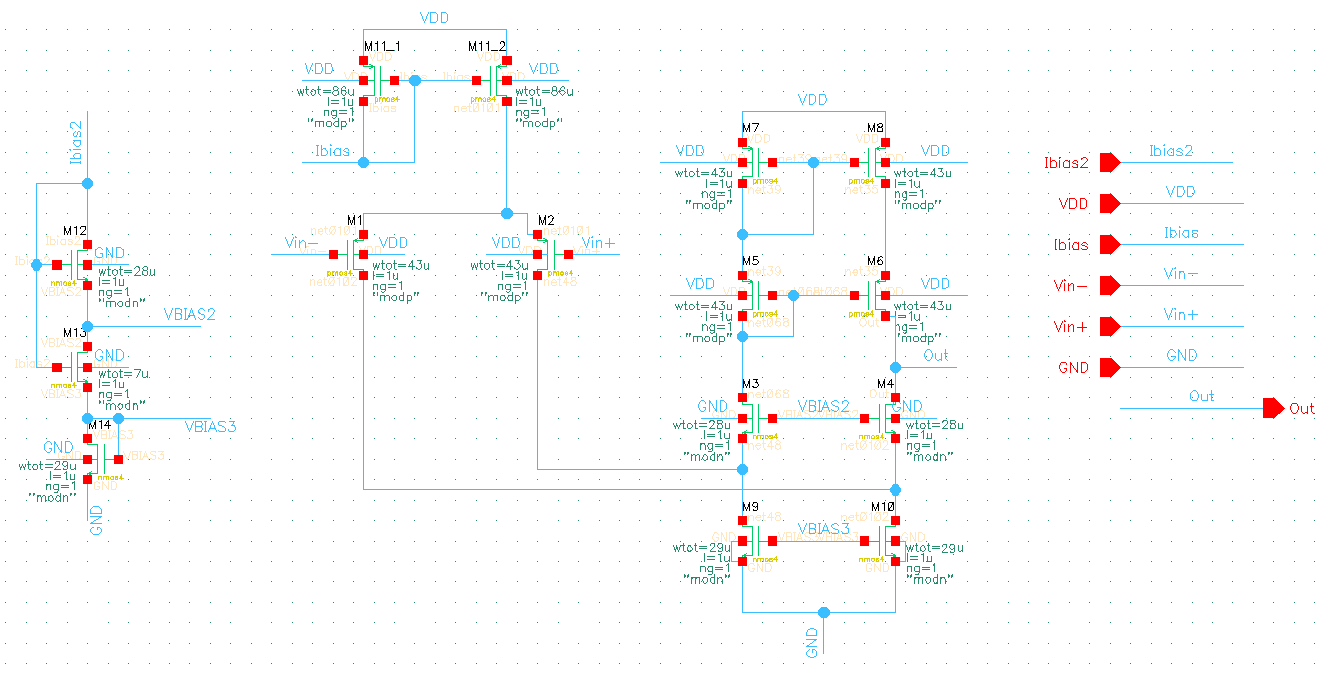
\includegraphics[keepaspectratio=true, scale=0.70]{exps/Wajustados}
	\vspace{-0.5em}
	\caption{\textit{Schematic} do circuito com os valores de $W$ ajustados.}
	\label{fig:ajustefail}
	\vspace{-0.8em}
\end{figure}

\begin{figure}[H]
	\centering
	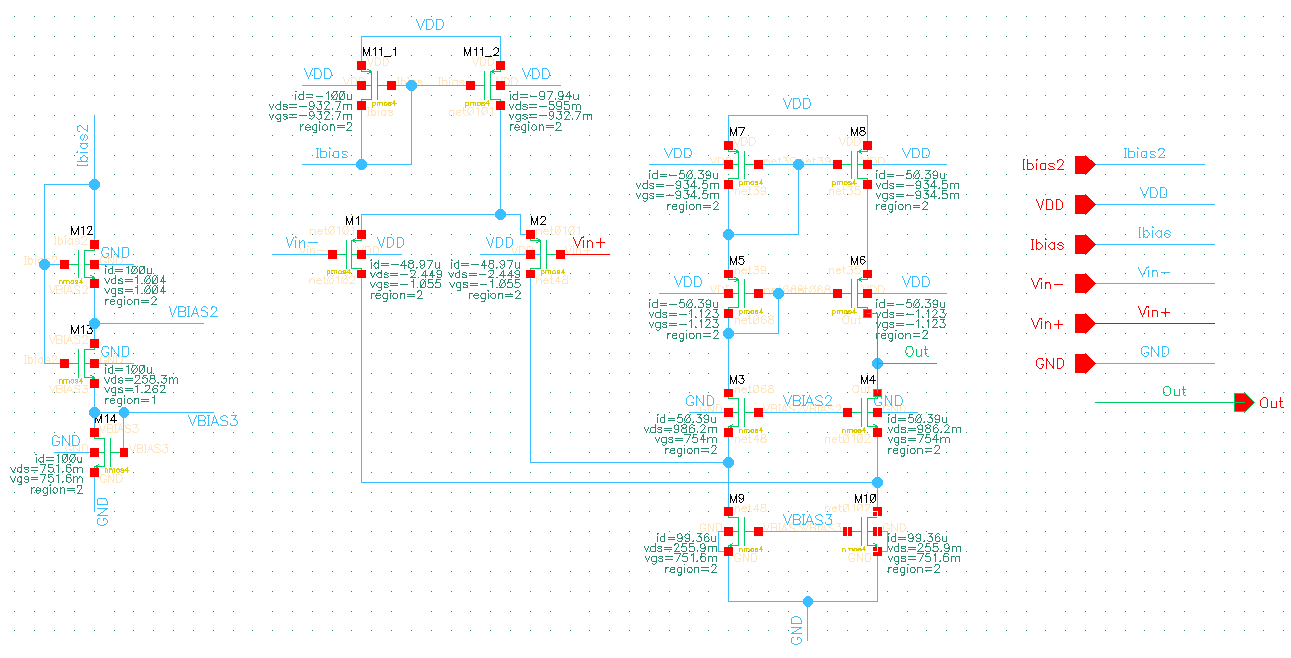
\includegraphics[keepaspectratio=true, scale=0.85]{exps/PFRajustados}
	\vspace{-0.5em}
	\caption{Valores do PFR do \textit{schematic} da Figura 9.}
	\vspace{-0.8em}
\end{figure}

Como se pode ver na figura anterior, o valor da corrente nos transístores M\textsubscript{3} a M\textsubscript{8} passou para 50.39 $\mu$A, um valor muito próximo do pretendido de 50 $\mu$A. Relativamente aos transístores M\textsubscript{9} e M\textsubscript{10}, passaram a ter uma corrente de 99.36 $\mu$A, um valor também bastante próximo do pretendido de 100 $\mu$A.

Face a estes ajustes mediu-se novamente o valor da \textit{slew-rate} para verificar se o critério já é cumprido. O valor medido foi de $199.9\times10^6$ V/segundo $\leftrightarrow 199.9$ V/$\mu$s, um valor que se considera óptimo.

Assim, o estado actual do circuito é apresentado de seguida. 

\begin{figure}[h]
	\centering
	\begin{minipage}[c]{0.58\textwidth}
		\begin{figure}[H]
			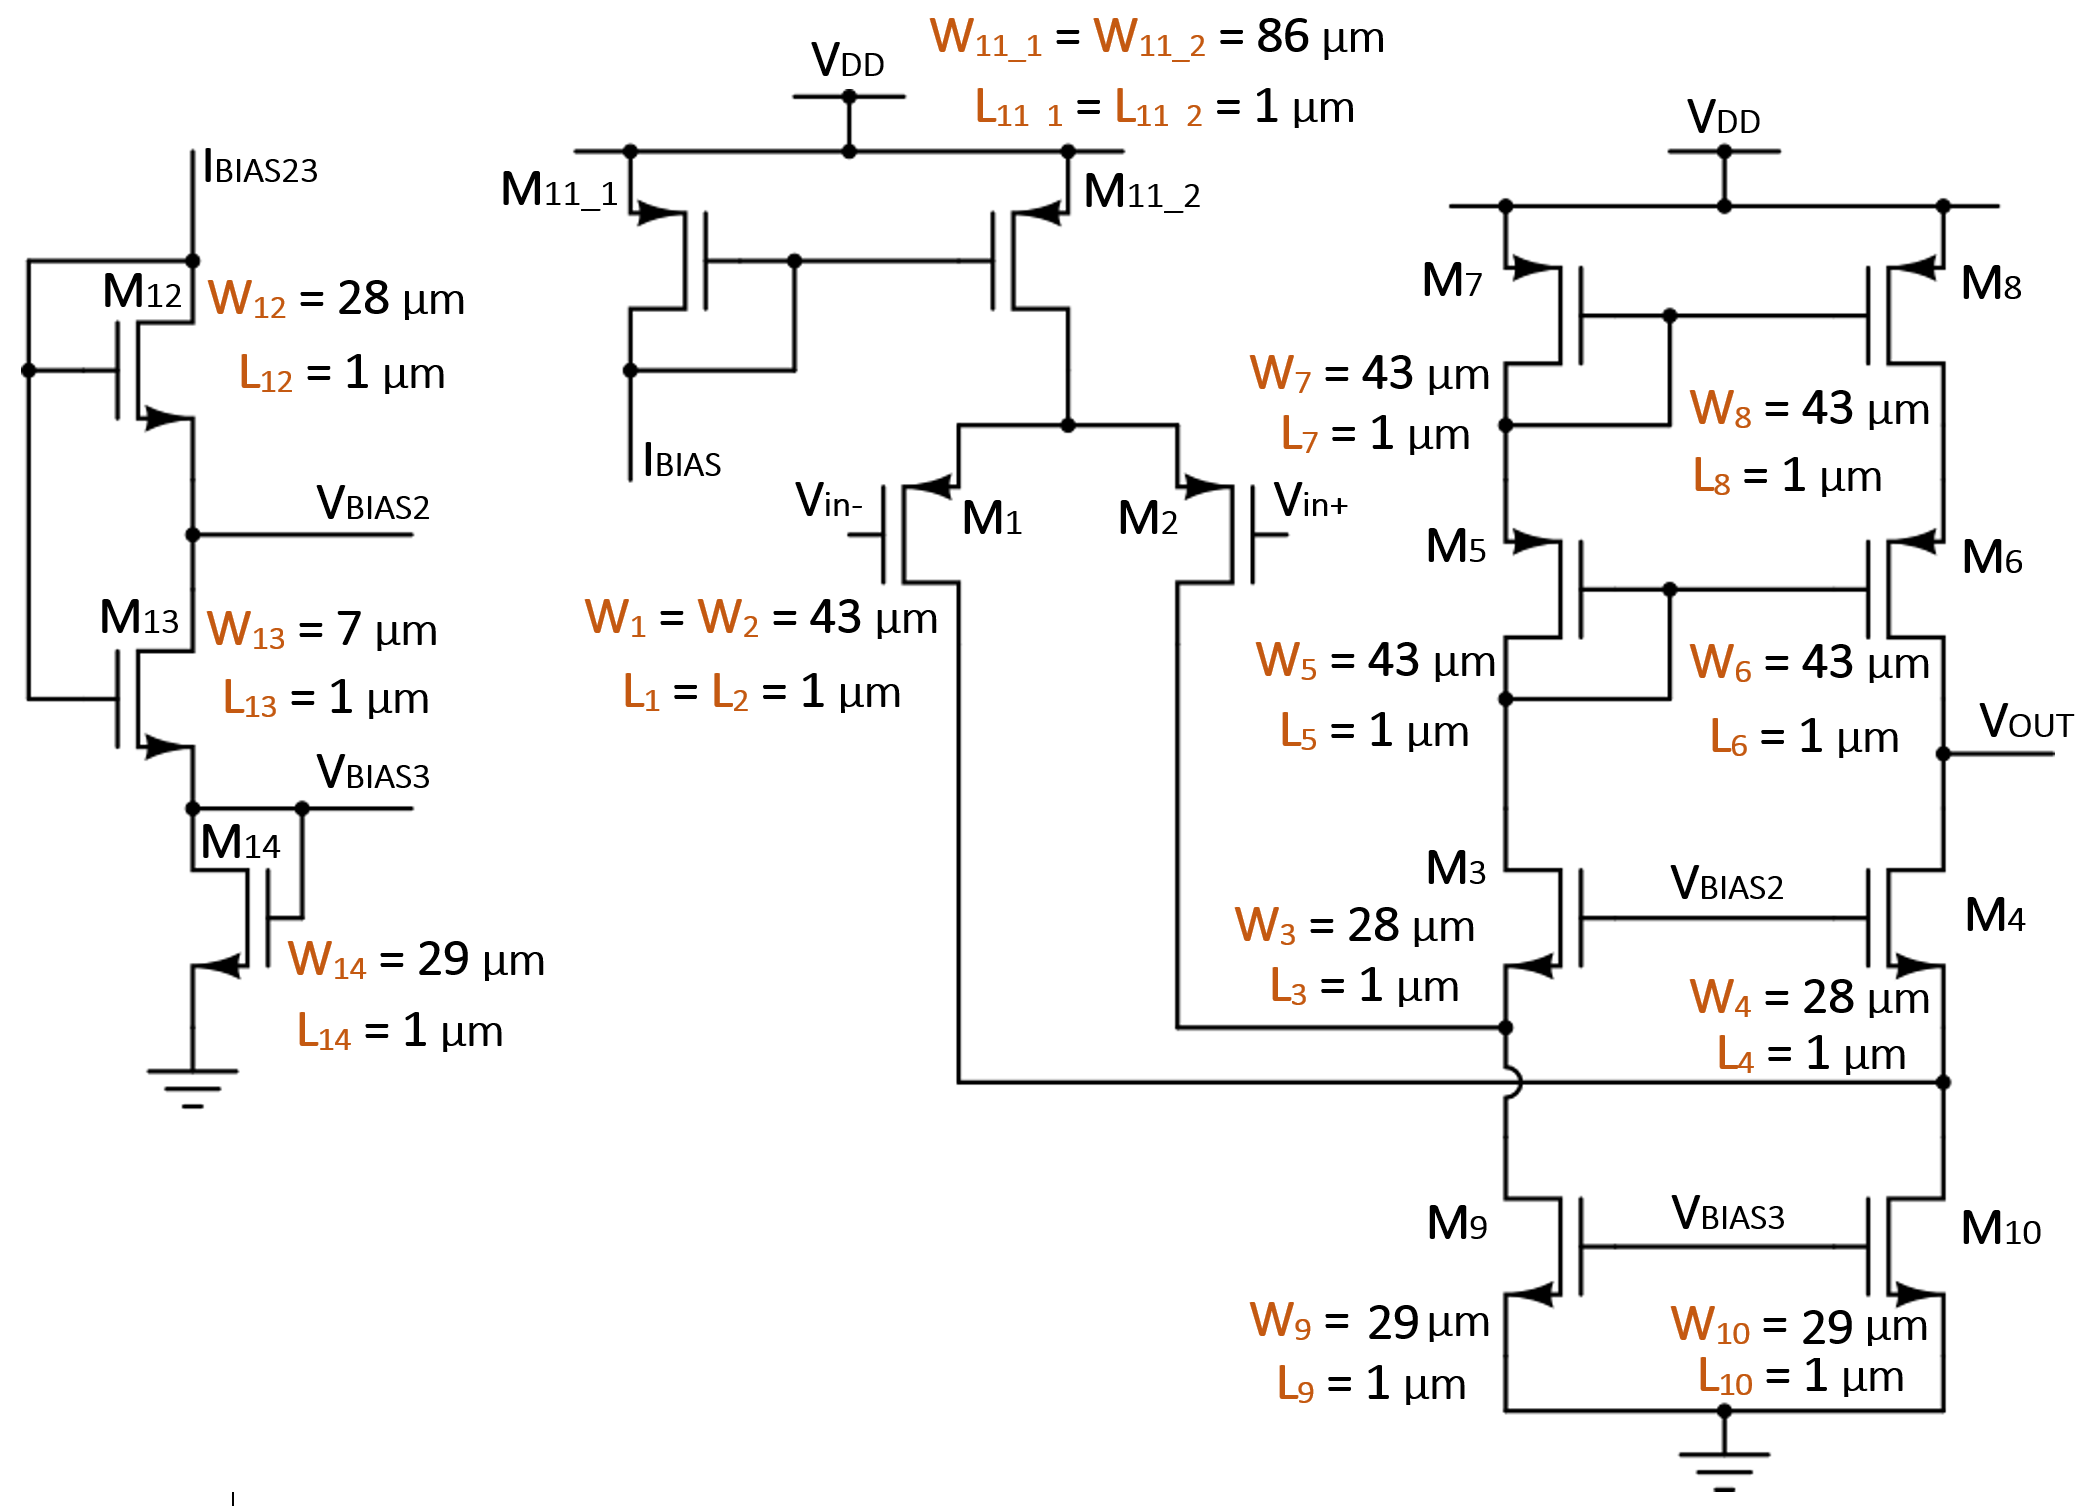
\includegraphics[keepaspectratio=true, scale=0.34]{teoricas/ajuste1}
			\caption{Circuito actual.}
			\vspace{-0.8em}
		\end{figure}
	\end{minipage}
	\begin{minipage}[c]{0.24\textwidth}
		\centering
		\begin{table}[H]
			\centering
			\caption{Especificações.}
			\vspace{-1.5mm}
			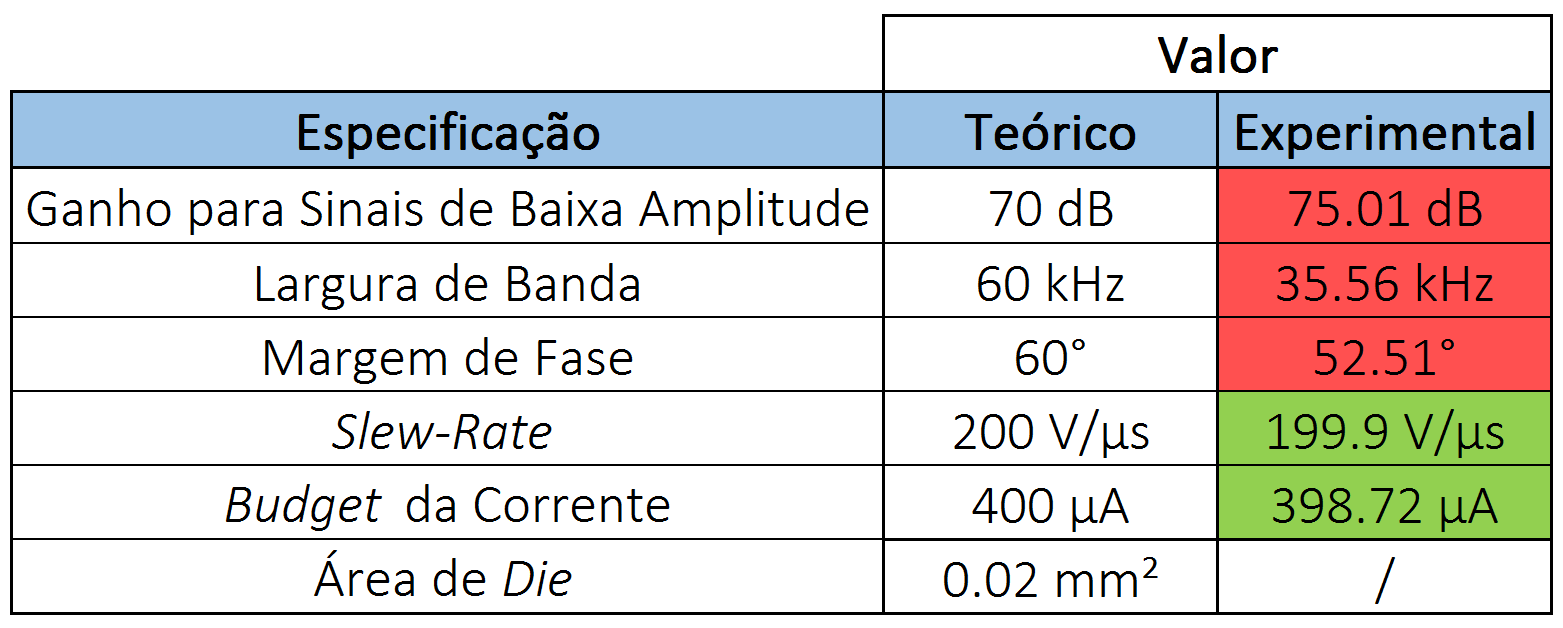
\includegraphics[keepaspectratio=true, scale=0.33]{teoricas/tabajuste1}
		\end{table}
	\end{minipage}	
\end{figure}

\vspace{-2mm}

\subsection{\textit{Slew-Rate}, Ganho, Largura de Banda e Margem de Fase}

Por análise da tabela anterior, verifica-se que o valor da largura de banda corresponde a metade do pretendido, sendo que depois se torna mais complicado conseguir recuperar sem comprometer a \textit{slew-rate} já obtida. 

Assim, optou-se por uma nova abordagem em que fica decidido não alterar o rácio $W/L$ dos transístores, com vista a não modificar o valor da sua transcondutância e não comprometer a sua região de funcionamento.

Olhando então para o primeiro ajuste feito, optou-se por modificar o valor de $L$ dos transístores M\textsubscript{3} e M\textsubscript{4} de maneira igual à modificação de $W$, ou seja, $L$ passa também para o dobro, ficando a 2 $\mu$m. Relativamente ao ajuste fino feito nos transístores M\textsubscript{12} e M\textsubscript{13}, opta-se por não manter o seu rácio $W/L$, algo que não é problemático, uma vez que não fazem parte do circuito do amplificador, mas sim parte de um circuito que o polariza em corrente. Face a esta modificação o circuito comporta-se da seguinte maneira. 

\vspace{-2mm}

\begin{figure}[H]
	\centering
	\begin{minipage}[c]{0.58\textwidth}
		\begin{figure}[H]
			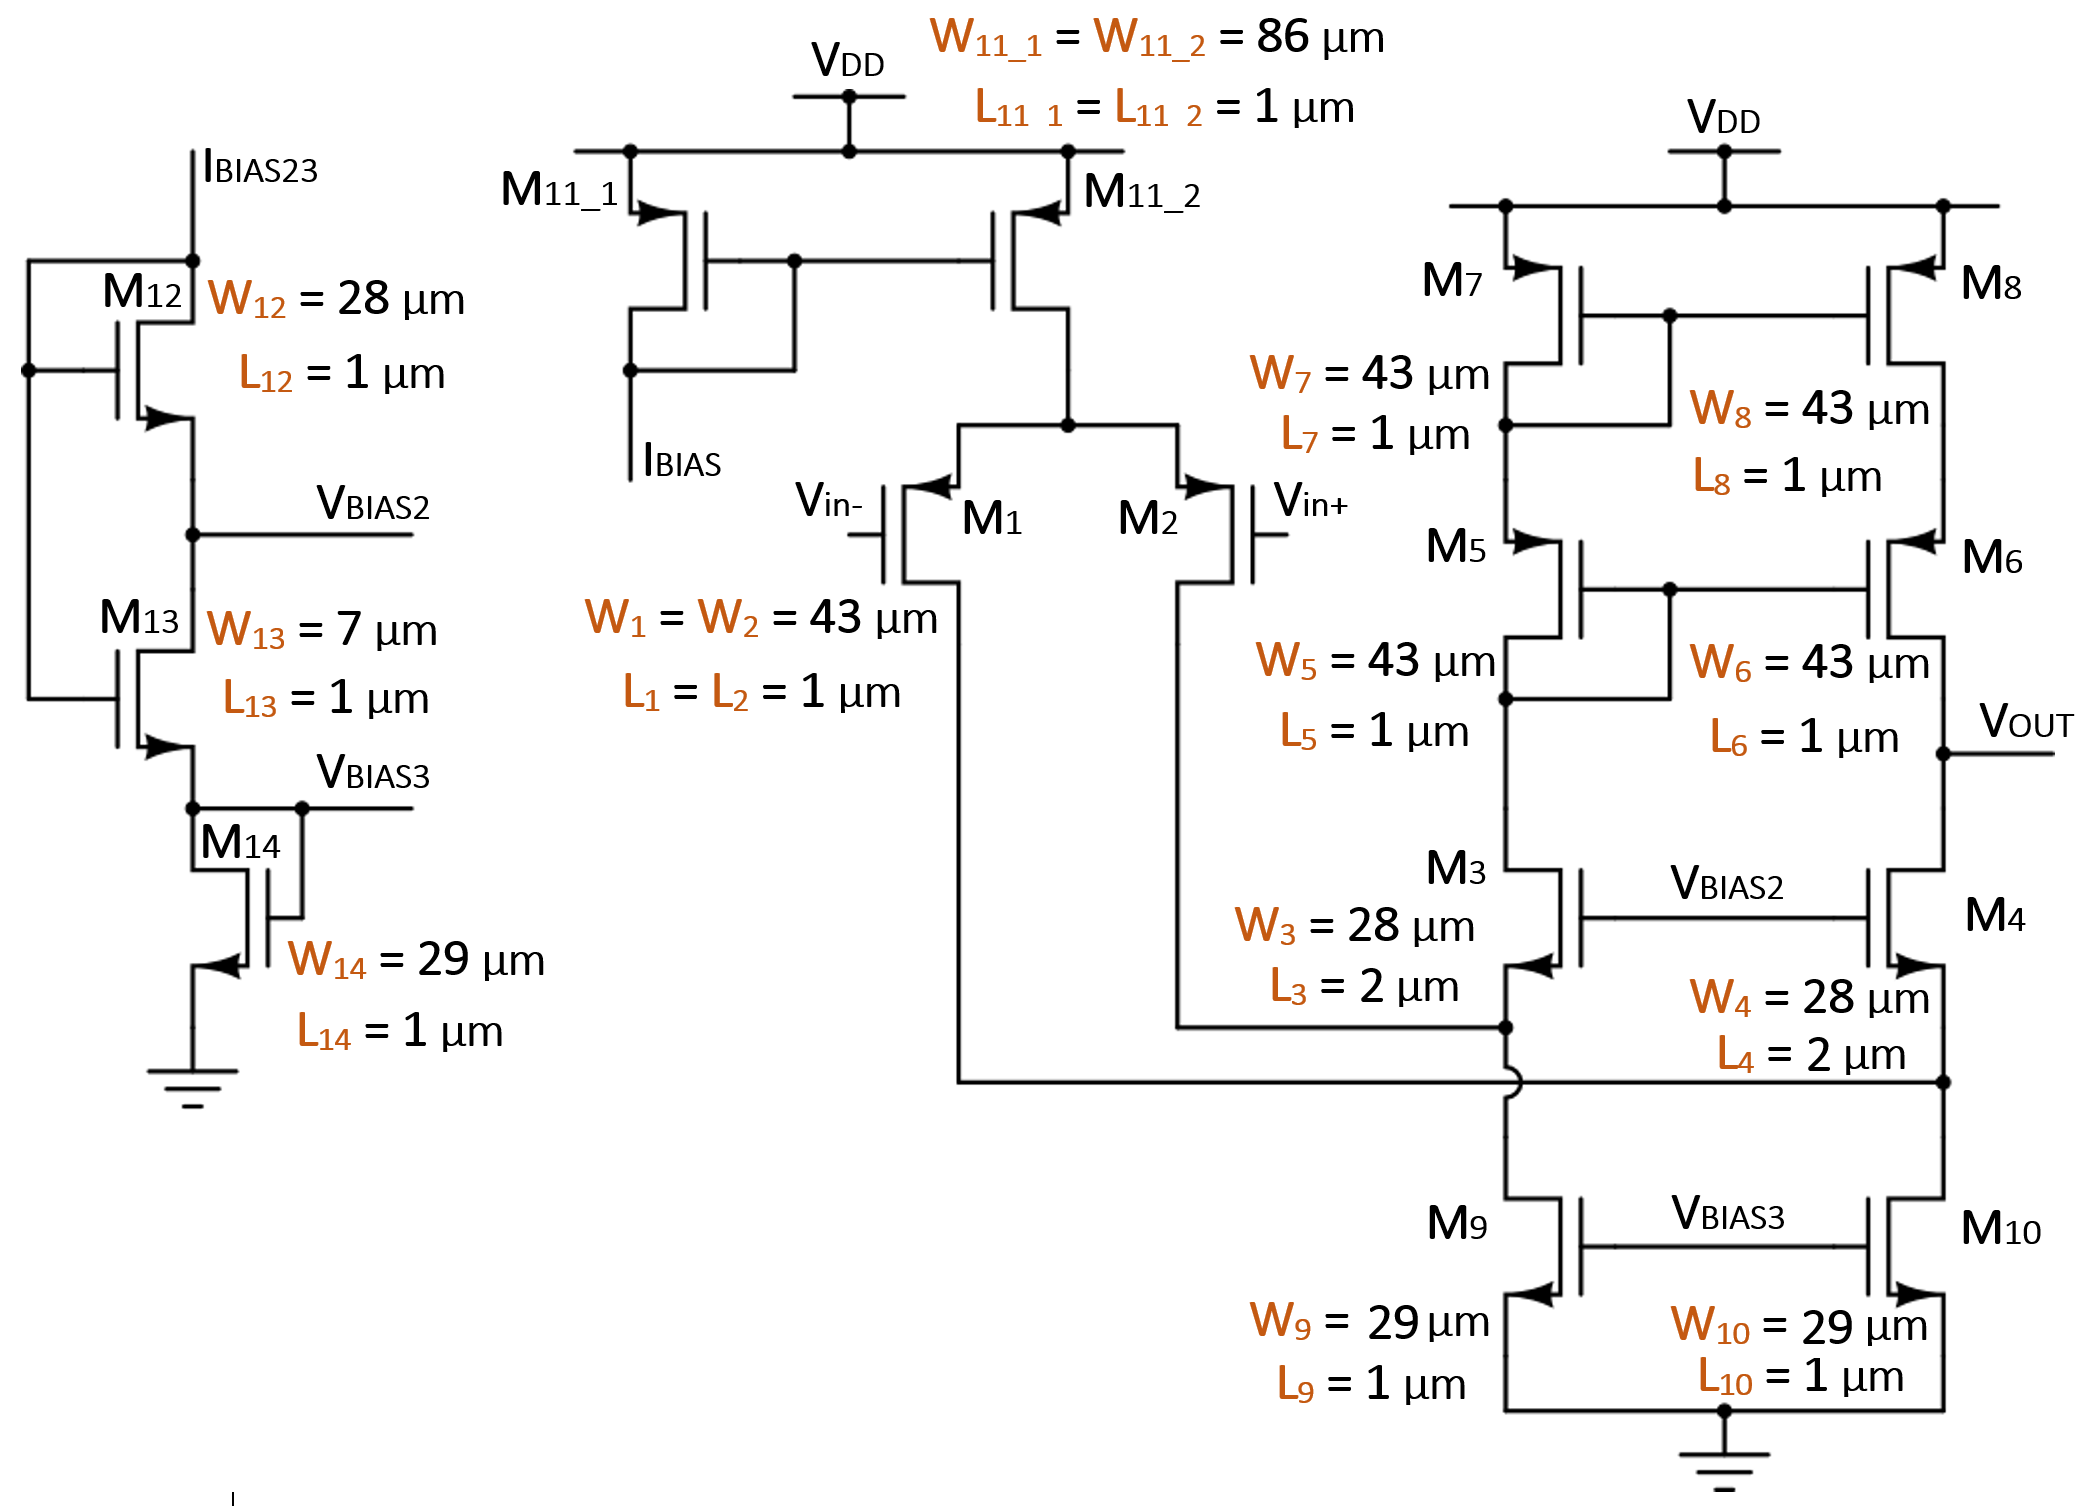
\includegraphics[keepaspectratio=true, scale=0.34]{teoricas/ajuste2}
			\caption{Circuito actual.}
			\vspace{-0.8em}
		\end{figure}
	\end{minipage}
	\begin{minipage}[c]{0.24\textwidth}
		\centering
		\begin{table}[H]
			\centering
			\caption{Especificações.}
			\vspace{-1.5mm}
			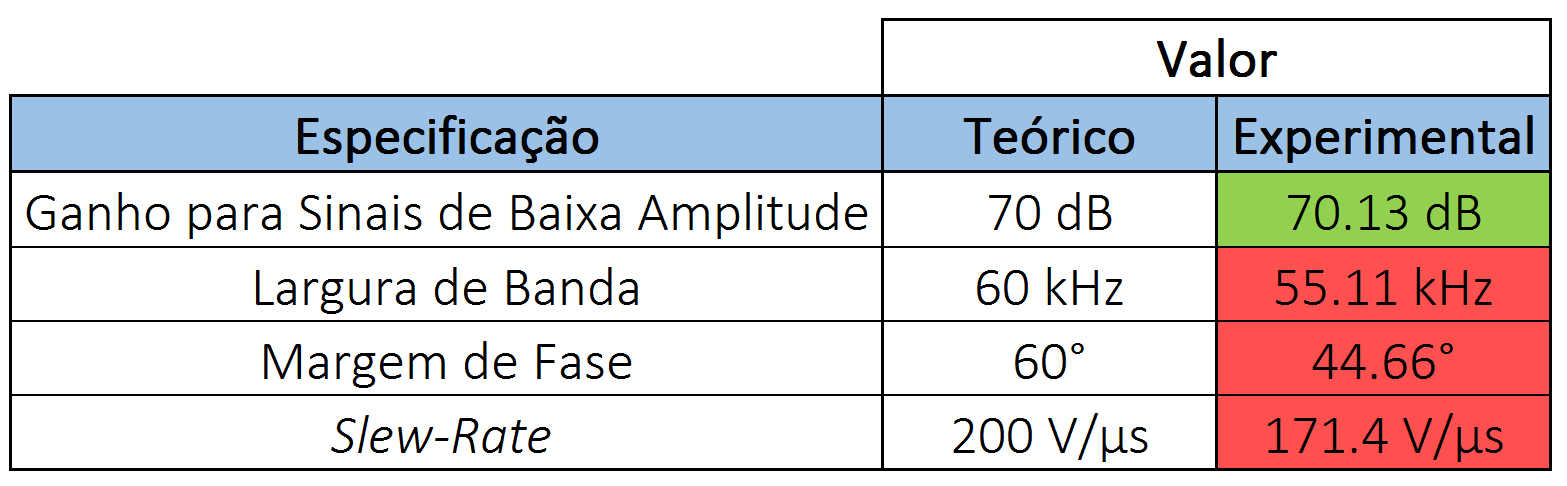
\includegraphics[keepaspectratio=true, scale=0.33]{teoricas/tabajuste2}
		\end{table}
	\end{minipage}	
\end{figure}

Como se pode ver pela Tabela 6, a \textit{slew-rate} desceu drasticamente face ao valor da Tabela 5. Assim, conclui-se que passar o rácio $W/L$ dos transístores M\textsubscript{3} e M\textsubscript{4} para o dobro é muito e optou-se por aumentar, numa primeira fase, em 30\% face ao valor original de $W = 14~\mu$m e $L = 1~\mu$m. Também nesta altura, verificou-se que considerar apenas o critério da \textit{slew-rate} como estando isolado dos demais critérios não é a melhor abordagem. De facto, optou-se por ter agora também em consideração o critério do ganho, da largura de banda e da margem de fase - tomou-se esta decisão pois uma análise teórica de todos estes factores revela o quão afectados são uns pelos outros.

Veja-se: o ganho do circuito é dado pela equação (3.10) e a largura de banda, que está associada à frequência do pólo dominante, é dada pela equação (3.11).

\vspace{-3mm}
\begin{equation}
A_{v} = g_{m_1} R_o =  g_{m_1}\left[\left(g_{m_4}r_{o_4}\left(r_{o_2}//r_{o_{10}}\right)\right)//\left(g_{m_6}r_{o_6}r_{o_8}\right)\right];
\end{equation}
\vspace{-2mm}
\begin{equation}
f_{p} = \frac{1}{2\pi C_L R_o} = \frac{1}{2\pi C_L \left[\left(g_{m_4}r_{o_4}\left(r_{o_2}//r_{o_{10}}\right)\right)//\left(g_{m_6}r_{o_6}r_{o_8}\right)\right]}.
\end{equation}

\vspace{4mm}

O parâmetro comum ao ganho e à largura de banda é $R_o$ - resistência de saída do amplificador \textit{folded cascode}. O valor de $R_o$ depende das resistências de saída de M\textsubscript{2} $\left(r_{o_2}\right)$, M\textsubscript{4} $\left(r_{o_4}\right)$, M\textsubscript{6} $\left(r_{o_6}\right)$, M\textsubscript{8} $\left(r_{o_8}\right)$ e M\textsubscript{10} $\left(r_{o_{10}}\right)$ e também da transcondutância de M\textsubscript{4} $\left(g_{m_4}\right)$ e M\textsubscript{6} $\left(g_{m_6}\right)$. 

O valor da transcondutância é directamente proporcional ao rácio $W/L$ e a resistência de saída de um transístor é dada por:

\vspace{-3mm}
\begin{equation}
r_{o} = \left[\lambda \frac{1}{2}\mu_{n}C_{ox}\times \left(\frac{W}{L}\right) \times \left(V_{GS}-V_{TH}\right)^2\right]^{-1}.
\end{equation}

\vspace{1mm}
Sabendo que se procura sempre manter o rácio das dimensões dos transístores vem:

\vspace{-3mm}
\begin{equation}
g_{m}: ~\text{aumentar/diminuir}~W~\text{e}~\text{aumentar/diminuir}~L \rightarrow~\text{mantém valor}~de~g_{m}
\end{equation}
\begin{equation}
r_{o}:  \begin{cases} ~\text{aumentar}~W~\text{e}~\text{aumentar}~L \rightarrow~\text{aumenta valor de}~de~r_{o} \\ ~\text{diminuir}~W~\text{e}~\text{diminuir}~L \rightarrow~\text{diminui valor de}~de~r_{o} \end{cases}
\end{equation}

A margem de fase, $PM$, é afectada pela frequência do pólo não dominante, sendo dada pela equação (3.15), tal como se pode ver de seguida.

\vspace{-3mm}
\begin{equation}
f_{np} = \frac{g_{m_3}}{2\pi C_{n_1}} \approx \frac{g_{m_3}}{2\pi \left[C_{gs_3} + C_{db_2} + C_{db_9}\right]}.
\end{equation}

\vspace{3mm}
Analisando a equação anterior tem-se quatro graus de liberdade: $g_{m_3}$, $C_{gs_3}$, $C_{db_2}$ e $C_{db_9}$. Como foi referido anteriormente, o rácio $W/L$ mantém-se, logo o valor de $g_{m_3}$ é constante. Assim, os parâmetros que afectam de facto a frequência do pólo não dominante são $C_{gs_3}$, $C_{db_2}$ e $C_{db_9}$. De seguida apresentam-se as equações que definem $C_{gs}$ e $C_{db}$ em função de $W$, $L$ e $V_{DB}$.

\unsure{nao sera melhor dizer o que é cada condensador daqueles? se dizemos que gm é a transcondutancia é melhor dizer tambem o que sao os condesandores}

\vspace{-3mm}
\begin{equation}
C_{gs} = \frac{2}{3} W L C_{ox};
\end{equation}
\vspace{-2mm}
\begin{equation}
C_{db} = \frac{C_{db0}}{\sqrt{1 + \frac{V_{DB}}{V_0}}};
\end{equation}
	
\vspace{1mm}

\begin{equation}
	PM: ~\text{aumentar}~f_{np}\rightarrow~\text{diminui valor de}~PM;
\end{equation}
\begin{equation}
f_{np}:  \begin{cases} ~\text{aumentar}~W~\text{e}~\text{aumentar}~L \rightarrow~\text{aumenta valor de}~C_{gs} \rightarrow~\text{diminui valor de}~f_{np} \\ ~\text{aumentar}~V_{DB} \rightarrow~\text{diminui valor de}~C_{db} \rightarrow~\text{aumenta valor de}~f_{np}\end{cases}
\end{equation}

\vspace{3mm}

As tensões $V_{DB_2}$ e $V_{DB_9}$ são dadas pelas seguintes equações:
	\vspace{-3mm}
	\begin{equation}
	V_{DB_2} = V_D - V_B = V_{DD} - R_{2} I_D - V_{DD} = - R_{o_{11\_2}} I_D ;
	\end{equation}
	\begin{equation}
	V_{DB_9} = V_D - V_B = V_{DD} - R_{9} I_D - GND = V_{DD} - R_{o_9} I_D ;
	\end{equation}
	
\vspace{1mm}
Analisando o circuito observa-se que a resistência $R_{2}$ depende da resistência de saída do transístor  M\textsubscript{11\textsubscript{1}}, ou seja de $r_{o_{11\_2}}$. A resistência $R_{9}$ depende dos transístores M\textsubscript{2}, M\textsubscript{3}, M\textsubscript{5} e M\textsubscript{7}. Veja-se:
	
\vspace{-3mm}
\begin{equation}
R_{9} = \left(g_{m_2}r_{o_2}\right)//\left(g_{m_3}r_{o_3}r_{o_5}r_{o_7}\right);
\end{equation}

\todo{falar agora de como se juntou toda esta logica para produzir a tabela}

\info{pode ajudar a explicar - na tabela estava: na iteraçao 3 houve uma ma alteraçao e voltou-se atras. na iteraçao 21 houve um ajuste de gm3 e gm4}
	
Os rácios de $W/L$ que se procura manter são apresentados na seguinte tabela.

\begin{table}[H]
	\centering
	\caption{Rácios das dimensões dos transístores que constituem o amplificador.}
	\vspace{-1.5mm}
	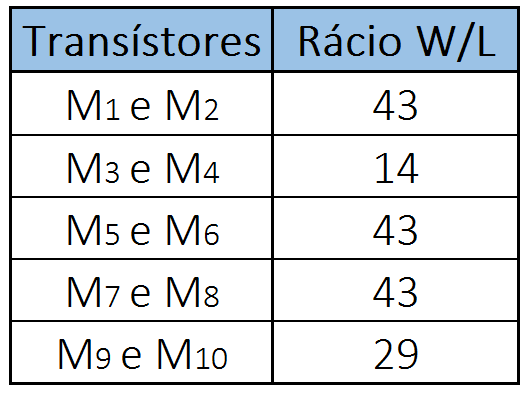
\includegraphics[keepaspectratio=true, scale=0.33]{teoricas/racios}
\end{table}

De seguida apresenta-se uma tabela que representa a linha temporal das mudanças que foram sendo feitas nas dimensões dos transístores de acordo com a lógica anteriormente explicada. Cada célula da tabela corresponde a um rácio $W/L$ do par de transístores correspondente e, para cada alteração feita numa determinada iteração, representa-se também o actual valor das especificações que se pretende cumprir.

De referir que, os transístores são sempre modificados aos pares, ou seja, um ajuste em M\textsubscript{1} implica igual ajuste em M\textsubscript{2}, sendo o mesmo válido para M\textsubscript{3} e M\textsubscript{4}, M\textsubscript{5} e M\textsubscript{6}, M\textsubscript{7} e M\textsubscript{8} e ainda para M\textsubscript{9} e M\textsubscript{10}. Isto feito para que o circuito não fique em desiquilíbrio.

\begin{table}[H]
	\centering
	\caption{Linha temporal das alterações nas dimensões dos transístores e valores experimentais registados.}
	\vspace{-1.5mm}
	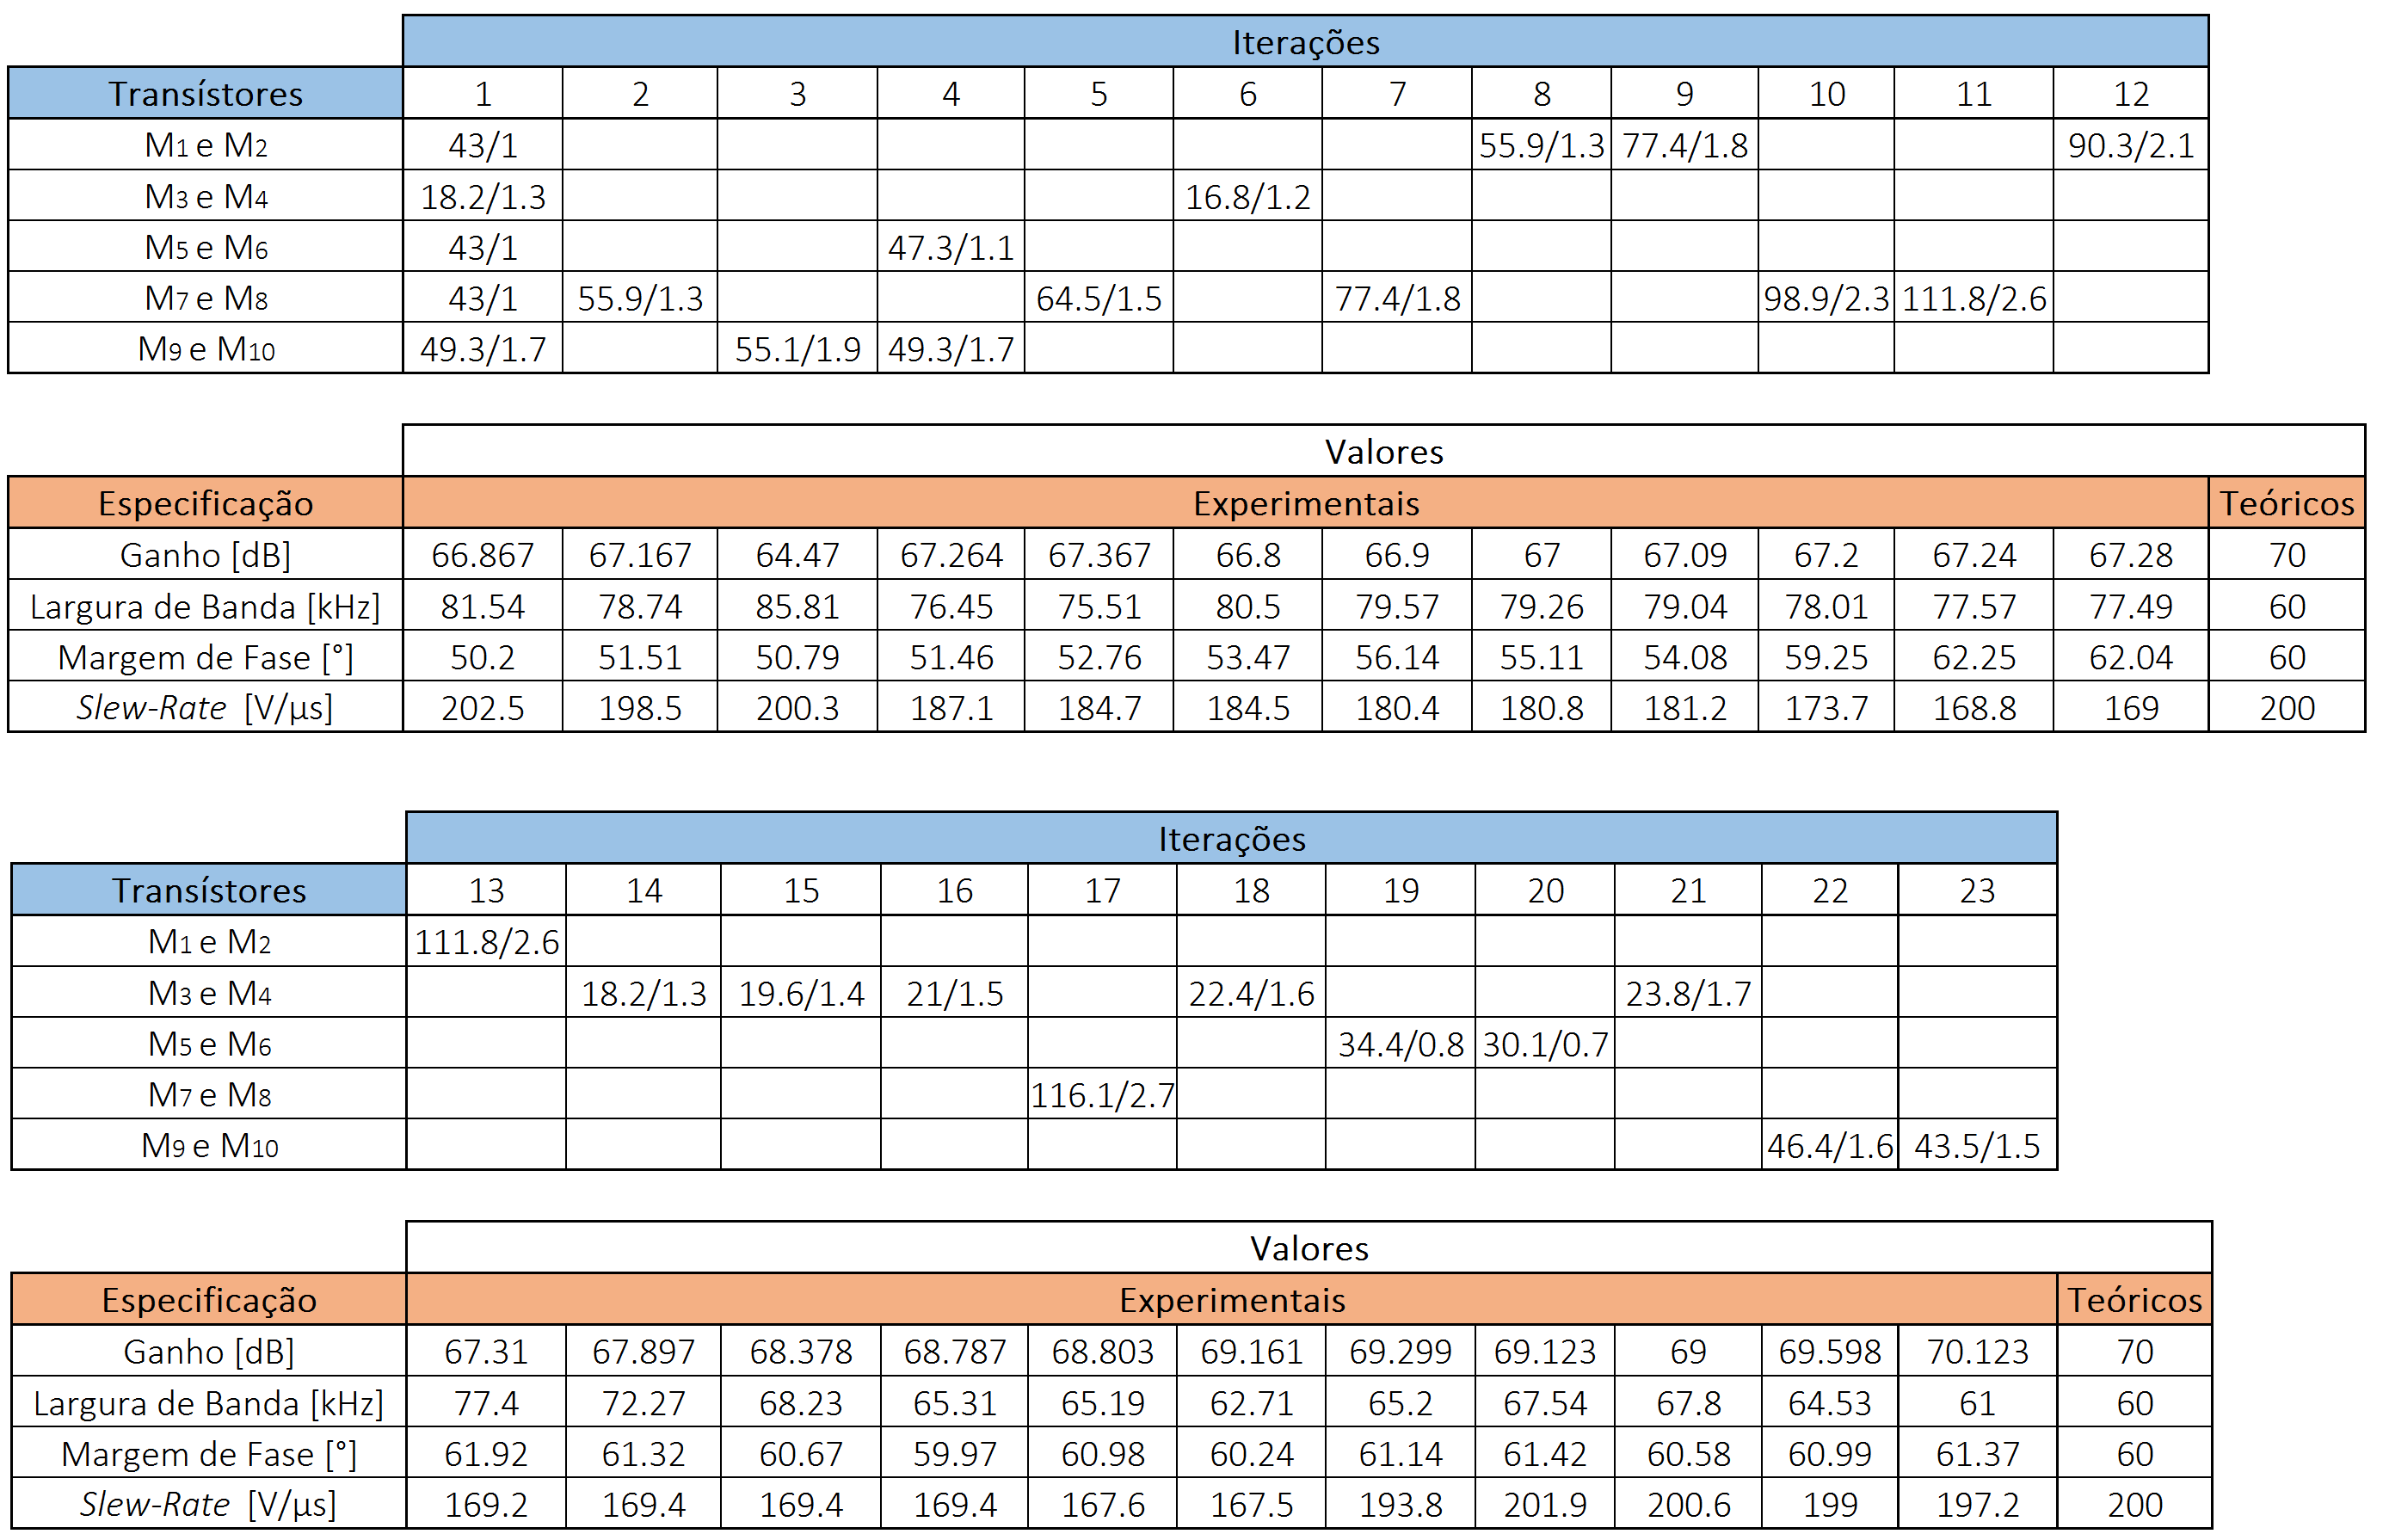
\includegraphics[keepaspectratio=true, scale=0.40]{teoricas/tabelaF1}
\end{table}

Como se pode ver, quando se atinge última iteração as especificações estão bastante próximas do pretendido e o circuito que permite atingir estas as especificações determinadas anteriormente é:

\begin{figure}[H]
	\centering
	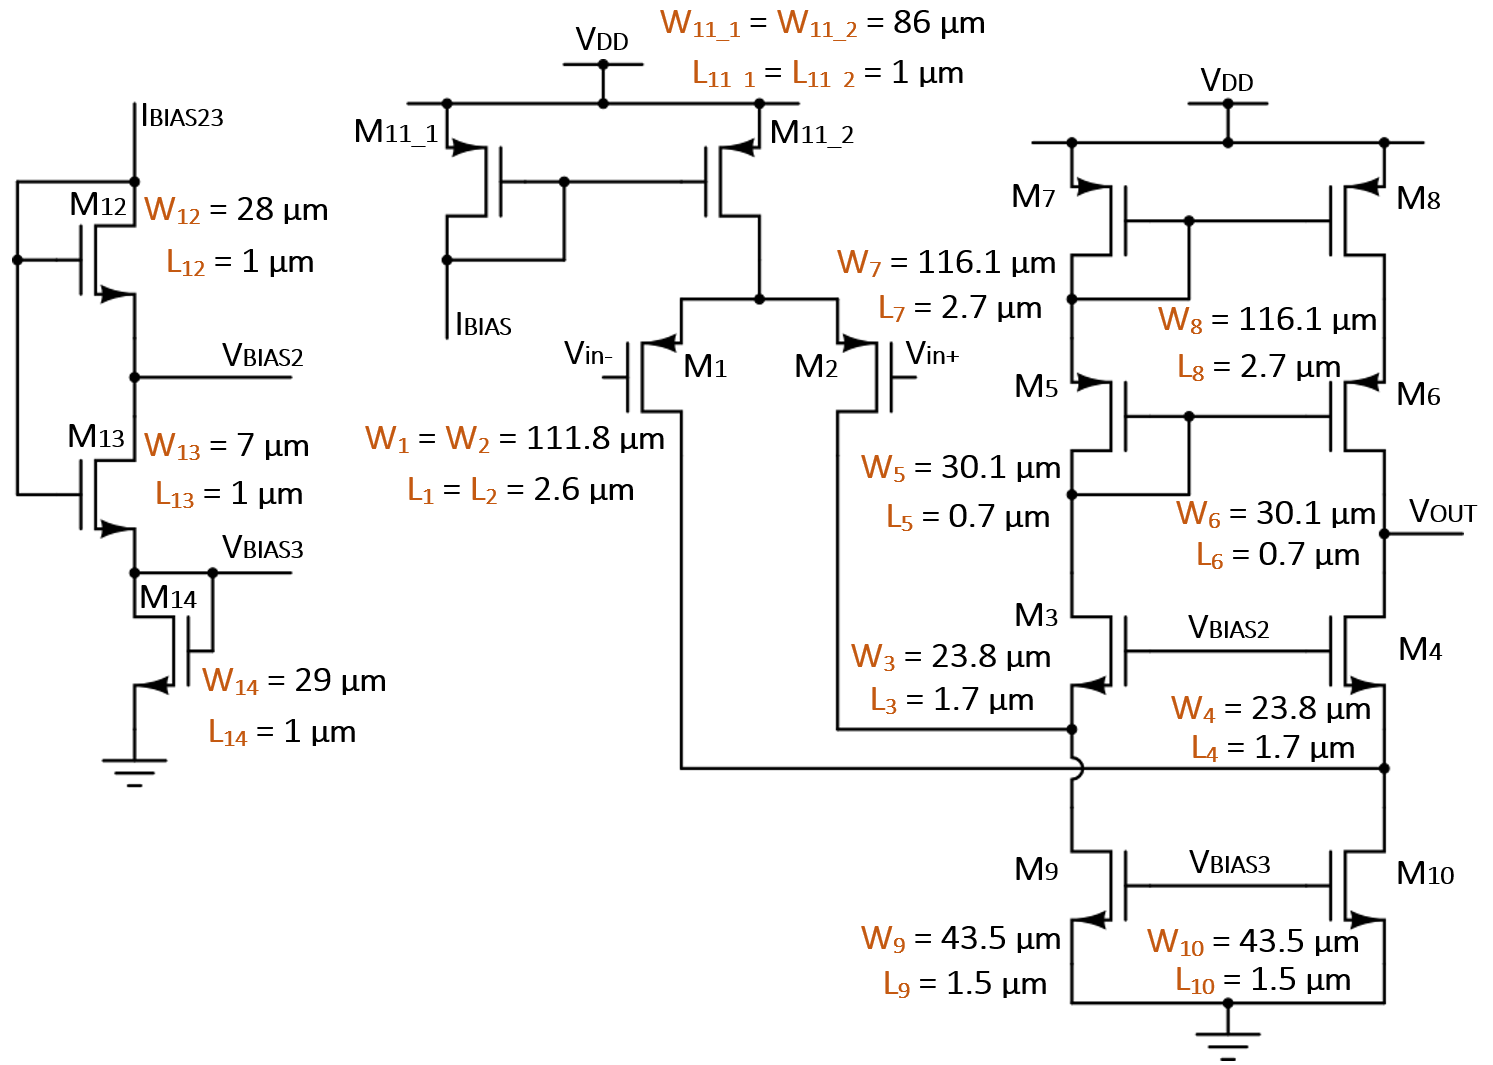
\includegraphics[keepaspectratio=true, scale=0.70]{teoricas/ajustesF1}
	\vspace{-0.5em}
	\caption{Circuito actual.}
	\vspace{-0.8em}
\end{figure}

\begin{table}[H]
	\centering
	\caption{Especificações actuais do circuito.}
	\vspace{-1.5mm}
	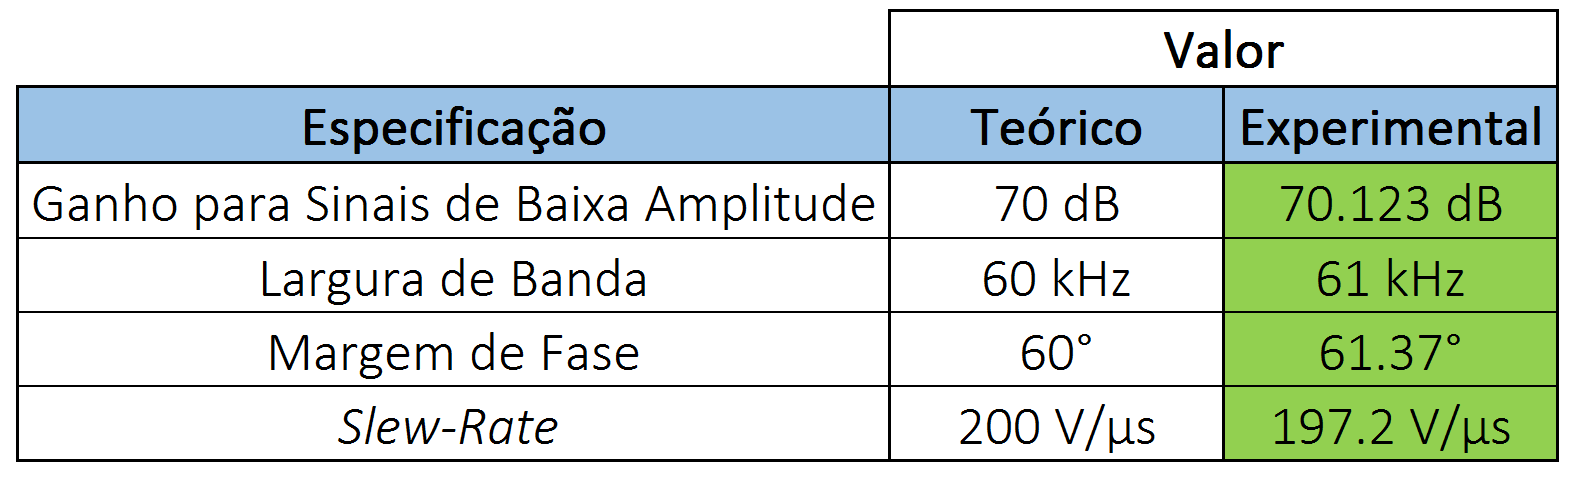
\includegraphics[keepaspectratio=true, scale=0.40]{teoricas/specsajustesF1}
\end{table}

\unsure{ultrapassamos budget da corrente, mas nao faz mal porque depois vamos mudar. por isso vou manter na mesma e depois ate me ajuda a explicar na seccao seguinte}

Na Figura 16 encontra-se o \textit{schematic} criado no Cadence correspondente ao da Figura 15.

\begin{figure}[H]
	\centering
	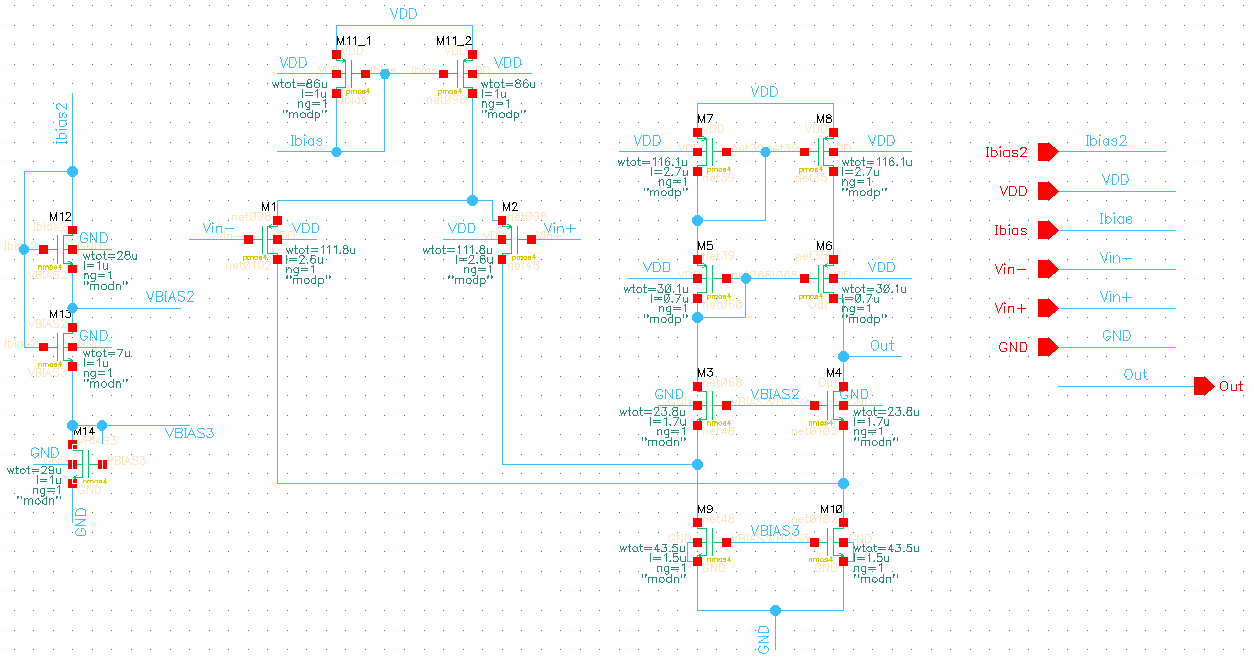
\includegraphics[keepaspectratio=true, scale=0.75]{exps/schematicajustesF1}
	\vspace{-0.5em}
	\caption{\textit{Schematic} do circuito actual.}
	\vspace{-0.8em}
\end{figure} 

Apresenta-se de seguida as simulações obtidas com o Cadence.

\begin{figure}[H]
	\centering
	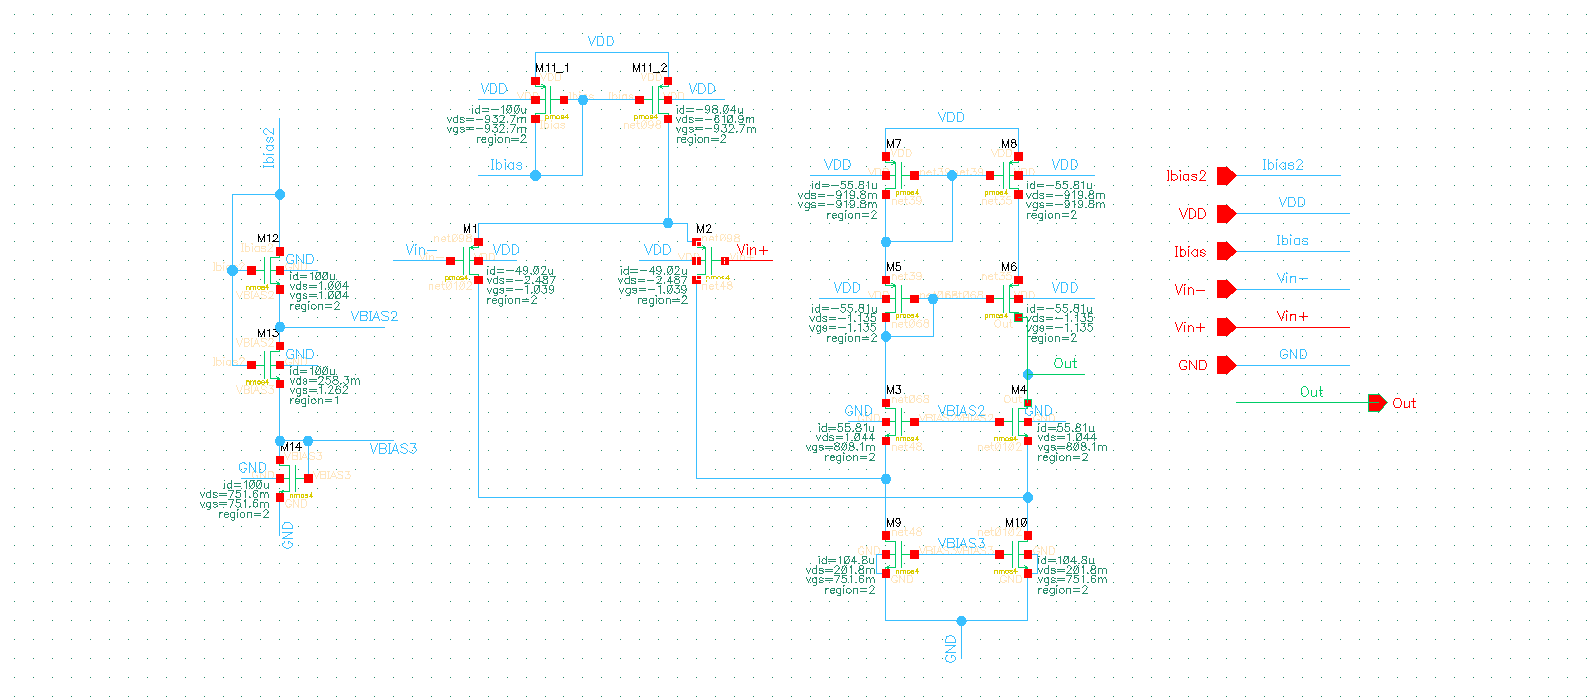
\includegraphics[keepaspectratio=true, scale=0.85]{exps/PFRajustesF1}
	\vspace{-0.5em}
	\caption{Valores do PFR do \textit{schematic} da Figura 16.}
	\vspace{-0.8em}
\end{figure} 

\todo{graficos da simulação DC e AC}

\subsection{\textit{Budget} da Corrente}

Com as especificações associadas ao ganho, largura de banda, margem de fase e \textit{slew-rate} cumpridas, o foco vira agora para o \textit{budget} de corrente, de modo a que o consumo de corrente no circuito seja o mínimo possível. De facto, como se pode ver na Tabela 9, o \textit{budget} de corrente actual está acima do especificado e uma mudança no circuito é obrigatória.

Numa primeira abordagem para se corrigir este problema, opta-se por ``injectar'' uma corrente de 5$\mu$A na polarização de $V_{BIAS}$ e então ajustar a dimensão dos transístores do espelho de corrente básico, para que a corrente fornecida ao par diferencial seja de 100$\mu$A na mesma. Olhando apenas para o circuito do espelho de corrente vem:

\begin{figure}[H]
	\centering
	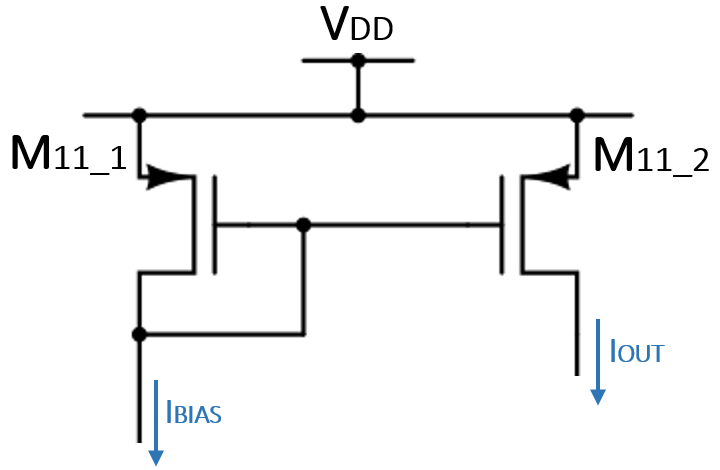
\includegraphics[keepaspectratio=true, scale=0.45]{teoricas/cmirror}
	\vspace{-0.5em}
	\caption{Espelho de corrente básico que polariza $V_{BIAS}$ em corrente.}
	\vspace{-0.8em}
\end{figure}

Do circuito anterior vem:

\vspace{-3mm}
\begin{equation}
	\frac{I_{OUT}}{I_{BIAS}} = \frac{\left(W/L\right)_{11_{2}}}{\left(W/L\right)_{11_{1}}};
\end{equation}

\vspace{1mm}
que permite concluir que a relação entre as duas correntes é controlada pela dimensão dos transístores. Pretende-se que $I_{BIAS}$ seja 5 $\mu$A e que $I_{OUT}$ seja 100 $\mu$A.  

\todo{continuar esta mudanca de 100uA para 5uA}

\unsure{vamos tentar ajustar IBIAS2 que continua a 100uA?}

\pagebreak

\section{Área}

\todo{explicar como se fez para calcular a area e apresentar desenho e calculos}

\pagebreak

\section{Simulações de Monte Carlo e \textit{Corners}}

\unsure{vamos fazer isto?}

\pagebreak

\section{Conclusões}

\todo{sugiro: o Cadence funciona muito bem a partir de casa}

\pagebreak

\listoftodos[Notes]

\end{document}